% !TEX program = pdflatex
% Statistical Pharmacology via Kakutani Dichotomy IX
% Companion computations: code/exp09_ad_gamma_secretase_gsm.py, code/paper09_compute_tables.py
\documentclass[11pt,reqno]{amsart}

\usepackage[T1]{fontenc}
\usepackage[utf8]{inputenc}
\usepackage{lmodern}
\usepackage[a4paper,margin=27mm]{geometry}
\usepackage{amsmath,amssymb,amsthm,mathtools}
\usepackage{booktabs}
\usepackage{graphicx}
\graphicspath{{./}{../figures/}}
\usepackage{array}
\usepackage[expansion=false]{microtype}
\usepackage{enumitem}
\usepackage{xcolor}
\usepackage[colorlinks=true,linkcolor=blue!60!black,citecolor=blue!60!black,urlcolor=blue!60!black]{hyperref}

\theoremstyle{plain}
\newtheorem{theorem}{Theorem}[section]
\newtheorem{lemma}[theorem]{Lemma}
\newtheorem{proposition}[theorem]{Proposition}
\newtheorem{corollary}[theorem]{Corollary}
\theoremstyle{definition}
\newtheorem{definition}[theorem]{Definition}
\newtheorem{observation}[theorem]{Numerical observation}
\theoremstyle{remark}
\newtheorem{remark}[theorem]{Remark}
\numberwithin{equation}{section}

\newcommand{\CKI}{\mathrm{CKI}}
\newcommand{\Kcat}{K_{\mathrm{catalytic}}}
\newcommand{\CKItm}{\CKI_{\mathrm{TM}}}
\newcommand{\CKIcov}{\CKI_{\mathrm{cov}}}
\newcommand{\Snotch}{S_{\mathrm{Notch}}}
\newcommand{\dcone}{d_L^{\mathrm{cone}}}
\newcommand{\dconeeff}{d_L^{\mathrm{cone,eff}}}
\newcommand{\CC}{\mathcal{C}}
\newcommand{\GG}{\mathcal{G}}
\newcommand{\HH}{\mathcal{H}}
\newcommand{\MM}{\mathcal{M}}
\newcommand{\Ab}{\mathrm{A}\beta}
\newcommand{\kT}{k_{B}T}
\newcommand{\pkg}{\texttt{kakutani\_pharma}}
\newcommand{\lead}{\texttt{KMS-AD-309}}

\renewcommand{\abstractname}{Summary}
\setlength{\emergencystretch}{3em}
\raggedbottom

% Section 5 is a block of floats; let them pack densely instead of leaving half-empty pages.
\setcounter{topnumber}{4}
\setcounter{bottomnumber}{3}
\setcounter{totalnumber}{6}
\renewcommand{\topfraction}{0.96}
\renewcommand{\bottomfraction}{0.96}
\renewcommand{\textfraction}{0.04}
\renewcommand{\floatpagefraction}{0.70}

\title[Statistical pharmacology via Kakutani dichotomy IX]{Statistical Pharmacology via Kakutani Dichotomy IX:\\ Notch-Sparing $\gamma$-Secretase Modulators for Alzheimer's Disease, Schur-Complement Confinement of the Catalytic Block, and a Cone-Geodesic Model of Processive Trimming}

\author[Z. Chen]{Zhengyi Chen}
\address{Guangxi Key Laboratory of Drug Discovery and Optimization, School of Pharmacy, Guilin Medical University, Guilin 541199, P.~R. China}
\email{chenzhengyi@glmc.edu.cn}

\author[R. Chen]{Ruqing Chen}
\address{GUT Geoservice Inc., Montreal, Qu\'ebec, Canada}
\email{ruqing@hotmail.com}

\thanks{DOI: \href{https://doi.org/10.5281/zenodo.23051518}{10.5281/zenodo.23051518}.\newline Sources, code and data:\newline \url{https://github.com/Ruqing1963/kakutani-statistical-pharmacology-IX}. Papers I--VIII of the series are \cite{ChenChen2026I,ChenChen2026II,ChenChen2026III,ChenChen2026IV,ChenChen2026V,ChenChen2026VI,ChenChen2026VII,ChenChen2026VIII}, the integrating article is \cite{ChenChen2026S}, and the underlying monograph is \cite{Chen2026}.}
\thanks{This project was supported by the National Natural Science Foundation of China (No.~22464010), the Guangxi Natural Science Foundation of China (No.~2025GXNSFAA069294), and the 2025 Bagui Youth Top Talent Project.}
\date{30 September 2026}

\subjclass[2020]{Primary 92C40, 92C45; Secondary 62H12, 35J60, 15A18, 05C50}
\keywords{Kakutani index, $\gamma$-secretase, presenilin-1, Notch sparing, allosteric modulation, Schur complement, infinity-Laplacian, cone geodesic, elastic network, Alzheimer's disease}

\begin{document}

\begin{abstract}
Papers I--VIII built the Kakutani indices and their estimators. This is the first application to one target: the presenilin-1 core of $\gamma$-secretase, whose orthosteric inhibition failed in phase III because the enzyme also cleaves Notch. We seek a quadrant-II ligand of Paper~IV, silent at the active site and loud in the second-order index.
(1)~Taking block topology alone from the cryo-EM structures of $\gamma$-secretase bound to APP (\texttt{6IYC}), to Notch (\texttt{6IDF}) and to an inhibitor and a modulator at once (\texttt{7D8X}), we build a harmonic model with $D=300$ coordinates in a catalytic block of $30$, a TM6a/PAL gate of $70$ and a TM1--TM9 channel of $200$, whose stiffness is a graph Laplacian plus a tether, so $\lambda_{\min}=t=0.9000$ exactly.
(2)~Theorem~\ref{thm:schur} is the mechanism of quadrant~II: the catalytic block meets the machinery only through a weak coupling, so any perturbation of the machinery moves the catalytic precision by an amount exactly bilinear in that coupling, making the induced index second order and its covariance part fourth. A $64$-fold scan gives $1.9906$, $1.9709$, $1.9755$ and $3.9633$ against $2,2,2$ and $4$.
(3)~Theorem~\ref{thm:cone} solves the discrete infinity-Laplacian cone geodesic on the three-residue lattice, $\dcone=w\sum_{m\le k}m^{-1/2}$, to $4.44\times10^{-16}$; isotropy strictly minimises it at fixed total weight, so cooperativity must be shared across all three helices.
(4)~Proposition~\ref{prop:branch} treats the pathogenic line as branching at $E\cdot\Ab_{42}$ and derives \emph{both} clinical biomarkers from one partition, the law of the design brief being its strong-modulation limit, matched to $8.91\,\%$ across five compounds by one fitted constant.
(5)~Semagacestat lands in quadrant~IV (retention $13.31\,\%$, both biomarkers unmoved at $1.01\times$), Avagacestat also in~IV despite its Notch-sparing label ($5.8$ times the safety threshold), R-flurbiprofen in~III, and E2012 and the lead \lead{} in~II, with $\Ab_{42/40}$ down $2.37\times$ and $2.61\times$ as $\Ab_{38}/\Ab_{42}$ rises $2.82\times$ and $3.14\times$ at $99.9$ and $99.5\,\%$ retention.
(6)~The familial alleles L166P and E280A are modelled as losses of gate stiffness, not gains of activity; both rearrange the machinery as strongly as a drug and in the opposite direction, raising $R_{42/40}$ to $0.333$ and $0.344$. Both quadrant-II modulators reverse the clamp and return it to $0.135$--$0.156$, below the wild-type $0.182$, the stricter target $0.12$ needing $1.11$--$1.24$ times nominal occupancy. Neither inhibitor rescues at any occupancy, and Semagacestat delivers the whole Notch liability and none of the benefit.
(7)~The selectivity index saturates, ranking E2012 above the more potent lead; Proposition~\ref{prop:anti} separates the definitional from the empirical in an activity assay's $120$ hits out of $240$ ligands at $0\,\%$ recall on quadrant~II.
The model takes topology, not geometry, from the structures, compounds and alleles enter only through their class, and \lead{} is a designed point. Section~\ref{sec:assess} states five limits and five open problems.
\end{abstract}

\maketitle
\enlargethispage{\baselineskip}
\tableofcontents

%%%%%%%%%%%%%%%%%%%%%%%%%%%%%%%%%%%%%%%%%%%%%%%%%%%%%%%%%%%%%%%%%%%%%%%%%%%%%%%
\section{Introduction: the quadrant that the assay cannot see}
\label{sec:intro}

\subsection{A target that punishes potency}
$\gamma$-Secretase is an intramembrane aspartyl protease whose catalytic subunit is presenilin-1 \cite{Wolfe1999}. It performs the final cut that releases the amyloid-$\beta$ peptides from the C-terminal fragment of the amyloid precursor protein, and it does so processively \cite{Takami2009}: after an initial $\epsilon$-cut it trims the substrate in steps of three residues along two parallel product lines,
\begin{equation}
\label{eq:lines}
\Ab_{49}\to\Ab_{46}\to\Ab_{43}\to\Ab_{40}
\qquad\text{and}\qquad
\Ab_{48}\to\Ab_{45}\to\Ab_{42}\to\Ab_{38},
\end{equation}
the first from an $\epsilon$-cut at Leu49 and the second from one at Thr48. What matters clinically is not how much $\Ab$ the enzyme makes but which species it releases, because the aggregation propensity of the products is steeply graded: $\Ab_{42}$ nucleates, $\Ab_{40}$ and $\Ab_{38}$ largely do not. The pathogenic observable is a ratio, not a rate, and the two ratios reported from trials, $\Ab_{42}/\Ab_{40}$ and $\Ab_{38}/\Ab_{42}$, are both read-outs of where the second line in \eqref{eq:lines} stops.

The same enzyme also performs the S3 cut that liberates the Notch intracellular domain. An orthosteric inhibitor occupies the catalytic aspartate dyad, D257 on TM6 and D385 on TM7, and therefore suppresses both substrates at once. That is the arithmetic behind the failure of Semagacestat: a compound that inhibited $\gamma$-secretase exactly as designed, and whose phase III trials were stopped for worsened cognition and for toxicities consistent with loss of Notch signalling. Reducing total $\Ab$ by shutting the enzyme down is not the same intervention as shifting the product distribution, and the clinical record has been unusually clear about the difference.

What is wanted instead is a \emph{modulator}: a ligand that leaves the dyad and the S3 register geometrically undisturbed and instead changes the register of processive trimming, so that the $\Ab_{42}$ line is pushed onward to $\Ab_{38}$. The first generation of such compounds, derived from non-steroidal anti-inflammatory drugs, was safe and too weak; R-flurbiprofen reached phase III and failed on efficacy. Safety and potency here are not a trade-off along one axis. They are two coordinates.

\subsection{What the cryo-EM structures fix}
\label{sec:cryoem}
Three structures from the Shi laboratory determine the anatomy this paper models, and it is worth being precise about which features are taken from them and which are not.

\emph{Substrate recognition, APP} \cite{Zhou2019}, PDB \texttt{6IYC}, $2.6$\,\AA. The transmembrane helix of the APP-C83 fragment is surrounded by five transmembrane helices of PS1, and one $\beta$ strand of APP joins two substrate-induced $\beta$ strands of PS1 into a hybrid $\beta$ sheet that positions the scissile bond. Residues at the PS1--APP interface are heavily enriched in familial-AD mutations, which is the structural statement behind Section~\ref{sec:fad}.

\emph{Substrate recognition, Notch} \cite{Yang2019}, PDB \texttt{6IDF}, $2.7$\,\AA. The Notch transmembrane helix is surrounded by three PS1 helices, and its C-terminal $\beta$ strand forms the same kind of hybrid sheet with two substrate-induced PS1 strands, on the intracellular side. PS1 rearranges pronouncedly on substrate binding. The two substrates therefore share not only the aspartate dyad but the register machinery that presents the scissile bond to it, which is exactly why an orthosteric inhibitor cannot separate them.

\emph{Inhibitor and modulator bound together} \cite{Yang2021}, PDB \texttt{7D8X}, $2.60$\,\AA. Human $\gamma$-secretase is resolved with the transition-state analogue L685,458 and the second-generation modulator E2012 bound \emph{simultaneously}. The inhibitor occupies the substrate-recruitment site on PS1; E2012 binds an allosteric site on the \emph{extracellular} side. That two ligands of opposite pharmacology occupy the same enzyme at once is the structural form of the two-coordinate picture this paper works in: potency at the active site and modulation of the machinery are not two ends of one axis.

What the model takes from these structures is the block topology only: that the catalytic dyad sits on TM6 (Asp257) and TM7 (Asp385); that a hybrid $\beta$ sheet with PS1 sets the cleavage register, which is what our catalytic block $\CC$ represents; that TM6a and the conserved PAL motif gate the advance of the substrate, which is our block $\GG$; and that TM1--TM9 form the horseshoe that encloses the substrate, which is our block $\HH$. What the model does \emph{not} take is geometry: no coordinates are used, no ligand is docked, and in particular the model does not place E2012 at the extracellular site that \texttt{7D8X} resolves. It represents a modulator by the coupling it induces between the gate and the channel, that is, by its consequence rather than its pose. Limit~(a) of Section~\ref{sec:assess} states this again.

\subsection{The four-quadrant reading}
Paper~IV introduced a classifier for ligands in the plane spanned by a local, pocket-visible perturbation and the second-order correlated Kakutani index $\CKI$, and observed that the pharmacologically interesting class sits where the first coordinate is small and the second is large: the ligand is invisible to a screen that watches the binding site, and loud in the covariance of the distal ensemble. Papers~V--VIII supplied the obstruction group, the cone-geodesic collective moves, the estimator pipeline \pkg{}, and the finite-sample calibration. All of that was developed on synthetic or generic systems.

This paper puts the machinery on one target and asks it to reproduce a known clinical separation. The two coordinates become concrete:
\begin{itemize}[leftmargin=1.6em,itemsep=2pt]
\item $\Kcat(L)$, the correlated Kakutani index between the apo and liganded ensembles restricted to the $30$ coordinates of the catalytic dyad and the Notch S3 register. This is the Notch-safety coordinate, and the design brief asks for $\Kcat<0.025$.
\item $\CKItm(L)$, the same index on the $270$ coordinates of the trimming machinery, the TM6a/PAL gate together with the TM1--TM9 channel. This is the potency coordinate, and the brief asks for $\CKItm>3.2$.
\end{itemize}
Quadrant~II is the conjunction. Quadrant~IV, high $\Kcat$ and low $\CKItm$, is the orthosteric inhibitor; quadrant~III, both low, is the silent analogue; quadrant~I, both high, is a potent ligand that has not escaped the Notch liability.

\subsection{Four results}
The paper contributes four things, in increasing order of what they cost to establish.

First, a \emph{mechanism} for why quadrant~II is reachable at all. Section~\ref{sec:model} builds a three-zone harmonic model of the catalytic core and Theorem~\ref{thm:schur} shows that the catalytic block is screened from the machinery at second order in the inter-block coupling. The screening is not an artefact of the perturbation being small: the perturbation is large, $\CKItm=4.25$ against a threshold of $3.2$, while what reaches the catalytic block is $\Kcat=1.7\times10^{-3}$. The Schur complement is the reason. A scan over the coupling scale confirms the predicted exponents to two decimal places.

Second, a \emph{geometry} for the three-residue step. Section~\ref{sec:cone} treats the synchronous displacement of TM3, TM6a and the PAL motif as a move from $(0,0,0)$ to $(1,1,1)$ on a three-bit lattice and computes its cost with the discrete infinity-Laplacian cone distance of Paper~VI. Theorem~\ref{thm:cone} gives the closed form for equal weights, $\dcone=w(1+2^{-1/2}+3^{-1/2})=2.284457\,w$, strictly below the sequential cost $3w$; the discount is what a modulator buys by making the three displacements cooperative. Proposition~\ref{prop:even} and Numerical observation~\ref{obs:mono} show that the discount is maximised exactly at the isotropic point, so a ligand that couples one helix strongly and the others weakly pays nearly the sequential price.

Third, a \emph{mechanism for the two clinical biomarkers}. Section~\ref{sec:branch} models the pathogenic product line as a branching process: at the intermediate $E\cdot\Ab_{42}$ the enzyme either releases the pathogenic peptide or performs one more synchronous three-residue cut to the benign $\Ab_{38}$. Proposition~\ref{prop:branch} derives both read-outs used in the clinic, $\Ab_{42}/\Ab_{40}$ and $\Ab_{38}/\Ab_{42}$, from that single partition, and shows that the phenomenological law of the design brief is its strong-modulation limit. The two biomarkers are then not independent observations but one number seen twice, which is what the trial data show.

Fourth, a \emph{calibration against the clinical record}, including familial disease. Section~\ref{sec:screen} places five compounds in the plane: Semagacestat and Avagacestat, both failed inhibitors; R-flurbiprofen, the failed first-generation modulator; E2012, representing the second-generation bridged-imidazole modulators that did lower CSF $\Ab_{42}$ and raise $\Ab_{38}$ while sparing Notch; and the designed lead \lead{}. It screens $240$ ligands, and examines what a conventional catalytic activity read-out does with them; Proposition~\ref{prop:anti} separates the part of that observation which is true by definition from the part which is an empirical property of the model. Section~\ref{sec:fad} then models two familial PSEN1 alleles, L166P and E280A, not as gains of activity but as losses of gate stiffness, and asks whether a quadrant-II modulator can undo them.

\subsection{What this paper does not do}
No structure is docked, no free energy is computed, and no molecule is synthesised. The dynamics are Gaussian and harmonic on a contact graph with the correct block topology, not molecular dynamics; the three compounds enter through three occupancy strengths rather than through their chemistry; and \lead{} is a point in that parameter space. The model reproduces a separation that is already known; it does not predict it from structure. Section~\ref{sec:assess} states this in detail, and everything in the paper is generated by two scripts whose acceptance tests are reproduced in Section~\ref{sec:tables}.

%%%%%%%%%%%%%%%%%%%%%%%%%%%%%%%%%%%%%%%%%%%%%%%%%%%%%%%%%%%%%%%%%%%%%%%%%%%%%%%
\section{A three-zone Gaussian elastic model and Schur-complement confinement}
\label{sec:model}

\subsection{The model}
\begin{definition}[Three-zone harmonic model]
\label{def:model}
Let $V$ be a set of $D=300$ harmonic degrees of freedom partitioned into fourteen segments, which are grouped into three blocks:
\begin{align*}
\CC \;&=\; \text{D257 loop }(8) \;\cup\; \text{D385 loop }(8) \;\cup\; \text{S3 register }(14), && |\CC|=30,\\
\GG \;&=\; \text{TM6a }(40) \;\cup\; \text{PAL }(30), && |\GG|=70,\\
\HH \;&=\; \text{TM1}\,(24),\dots,\text{TM9}\,(16), && |\HH|=200,
\end{align*}
and write $\MM=\GG\cup\HH$ for the trimming machinery, $|\MM|=270$. Let $G(L)$ be a weighted graph on $V$ whose edge weights depend on a ligand $L$, and let
\begin{equation}
\label{eq:K}
K(L) \;=\; \Lambda\bigl(G(L)\bigr) \;+\; t\,I_D,
\qquad t = 0.9,
\end{equation}
where $\Lambda$ is the weighted graph Laplacian. The conformational ensemble of $L$ is the Gaussian $N(\mu(L),\Sigma(L))$ with
\begin{equation}
\label{eq:ensemble}
\Sigma(L) = K(L)^{-1}, \qquad \mu(L) = \Sigma(L)\, f(L),
\end{equation}
in units of $\kT$, where $f(L)$ is the ligand binding force.
\end{definition}

The three blocks are the functional anatomy of Section~\ref{sec:cryoem}, coarse-grained. Block $\CC$ carries the aspartate dyad together with the register that the hybrid $\beta$ sheet imposes, which is what both substrates share and what the S3 cut on Notch requires; its three segments are the D257 loop on TM6, the D385 loop on TM7 and the S3 register itself. Block $\GG$ is the TM6a helix and the conserved P433--A434--L435 motif, the pair that gates the unwinding and advance of the substrate. Block $\HH$ is the TM1--TM9 horseshoe that encloses it.

The edges of $G$ are of three kinds. Inside each segment a backbone path carries weight $6.0$, $4.0$ or $5.0$ according to the block. Between segments there are packing contacts: nine consecutive helix-helix pairs plus three closures at weight $1.2$ inside the channel, TM6a--PAL at $1.5$, four gate-channel contacts at $1.0$, and three internal catalytic contacts at $0.8$. Finally, and decisively, the catalytic block meets the rest of the structure only through D257--TM6 and D385--TM7 at weight $0.35$ and S3 register--PAL at weight $0.25$. The placement of the two aspartates on TM6 and TM7 follows presenilin-1; the weakness of the three couplings is the design hypothesis whose consequences Theorem~\ref{thm:schur} draws out.

A ligand acts through three occupancy strengths $s_{\mathrm{cat}},s_{\mathrm{gate}},s_{\mathrm{chan}}\ge0$. The first adds springs across the dyad and the S3 register; the second couples TM6a to PAL and softens the TM6a backbone; the third creates cross-helix couplings TM3--TM6, TM3--TM7, TM5--TM9, TM2--TM8 and, critically, TM3--TM6a, while softening the TM3 and TM6 backbones. Each also contributes a binding force supported on its own block. Softening factors are floored at $0.15$, so every edge weight stays positive.

\begin{proposition}[Positive definiteness and the exact spectral floor]
\label{prop:pd}
For every ligand, $K(L)\succ0$ and $\lambda_{\min}(K(L))=t$ exactly, attained on the uniform direction $D^{-1/2}\mathbf{1}$. In particular $\dim\ker K=0$ and $\Sigma(L)$ is well defined.
\end{proposition}

\begin{proof}
All edge weights are positive, so $\Lambda(G)\succeq0$. The graph $G$ is connected, hence $\ker\Lambda(G)=\mathbb{R}\mathbf{1}$ and the second eigenvalue is positive. Adding $tI$ shifts the whole spectrum by $t$, so $\lambda_{\min}(K)=0+t=t$ with eigenvector $\mathbf{1}$, and every other eigenvalue exceeds $t$.
\end{proof}

The numerical spectrum of the apo model is $[0.9000,\,24.8622]$, condition number $27.62$, in agreement with Proposition~\ref{prop:pd}; see Table~\ref{tab:model}. The floor is attained, not approached, which is a useful invariant: any coding error that disturbed the Laplacian structure would move it.

\subsection{Indices}
Following Paper~II, for two Gaussians the correlated Kakutani index is the Bhattacharyya distance
\begin{equation}
\label{eq:cki}
\CKI = \underbrace{\tfrac18\,\Delta\mu^{\!\top}\bar\Sigma^{-1}\Delta\mu}_{D_{\mathrm{mean}}}
\;+\;\underbrace{\tfrac12\Bigl[\log\det\bar\Sigma-\tfrac12\bigl(\log\det\Sigma_A+\log\det\Sigma_B\bigr)\Bigr]}_{D_{\mathrm{cov}}},
\qquad \bar\Sigma=\tfrac12(\Sigma_A+\Sigma_B),
\end{equation}
and $D_{\mathrm{cov}}=D_{\mathrm{comm}}+D_{\mathrm{rot}}$ splits into a commuting spectral part and a non-negative eigenvector-rotation part. We write $\Kcat(L)$ for \eqref{eq:cki} evaluated on the marginals over $\CC$, and $\CKItm(L)$ for the same on $\MM$; $\CKIcov(L)$ denotes the covariance part of $\CKItm(L)$. A Gaussian marginal is the corresponding sub-block of $\Sigma$, so these are computed without any further approximation.

The Notch read-out is defined as follows. The S3 cut requires the correct register at three consecutive subsites, and we take each subsite to retain its register with probability equal to the Bhattacharyya affinity $e^{-\Kcat}$ of the catalytic ensembles. Hence
\begin{equation}
\label{eq:notch}
\text{Notch retention} \;=\; e^{-3\Kcat},
\end{equation}
so that the design threshold $\Kcat<0.025$ is exactly the statement that retention exceeds $e^{-0.075}=0.9277$.

\subsection{Schur-complement confinement}
Write the apo stiffness in block form and let $P$ denote the precision matrix of the catalytic marginal,
\begin{equation}
\label{eq:schur}
K=\begin{pmatrix}K_{\CC\CC} & K_{\CC\MM}\\ K_{\MM\CC} & K_{\MM\MM}\end{pmatrix},
\qquad
P \;=\; \Sigma_{\CC\CC}^{-1} \;=\; K_{\CC\CC}-K_{\CC\MM}K_{\MM\MM}^{-1}K_{\MM\CC}.
\end{equation}
An allosteric ligand, by definition, perturbs only the machinery: $\Delta K$ is supported on $\MM\times\MM$ and $f$ is supported on $\MM$.

\begin{theorem}[Second-order screening of the catalytic block]
\label{thm:schur}
Let $\Delta K$ be symmetric, supported on $\MM\times\MM$, with $K+\Delta K\succ0$, and let $f$ be supported on $\MM$. Then:
\begin{enumerate}[label=\textup{(\roman*)},leftmargin=2.2em,itemsep=3pt]
\item The catalytic precision changes by
\begin{equation}
\label{eq:dP}
\Delta P \;=\; -\,K_{\CC\MM}\Bigl[\bigl(K_{\MM\MM}+\Delta K_{\MM\MM}\bigr)^{-1}-K_{\MM\MM}^{-1}\Bigr]K_{\MM\CC},
\end{equation}
which is exactly bilinear in the coupling block $K_{\CC\MM}$. Consequently, if $K_{\CC\MM}$ is replaced by $sK_{\CC\MM}$ while $K_{\CC\CC}$ and $K_{\MM\MM}$ are held fixed, then $\Delta P=s^2\,\Delta P_1$ with $\Delta P_1$ independent of $s$, and $\|\Delta\Sigma_{\CC\CC}\|=O(s^2)$.
\item The catalytic mean displacement is
$\mu_\CC=-\Sigma_{\CC\CC}K_{\CC\MM}K_{\MM\MM}^{-1}f_\MM=O(s)$.
\item Therefore $D_{\mathrm{mean}}\bigl(\Kcat\bigr)=O(s^2)$ and $D_{\mathrm{cov}}\bigl(\Kcat\bigr)=O(s^4)$, so
$\Kcat=O(s^2)$, dominated at small $s$ by the mean term.
\item The index on the machinery, $\CKItm$, is unaffected to leading order: it depends on $K_{\CC\MM}$ only through $K_{\MM\MM}-K_{\MM\CC}K_{\CC\CC}^{-1}K_{\CC\MM}$, again an $O(s^2)$ correction to an $O(1)$ quantity.
\end{enumerate}
\end{theorem}

\begin{proof}
(i) An $\MM$-supported perturbation leaves $K_{\CC\CC}$ and $K_{\CC\MM}$ untouched, so subtracting the two instances of \eqref{eq:schur} cancels $K_{\CC\CC}$ and leaves \eqref{eq:dP}. The bracket depends on $s$ not at all, and $K_{\CC\MM}$ appears once on each side, giving the exact factor $s^2$. Since $\Sigma_{\CC\CC}=P^{-1}$ and $P\succ0$ uniformly, $\Delta\Sigma_{\CC\CC}=-P^{-1}\Delta P\,(P+\Delta P)^{-1}=O(\|\Delta P\|)=O(s^2)$.

(ii) The block-inverse formula gives $(K^{-1})_{\CC\MM}=-\Sigma_{\CC\CC}K_{\CC\MM}K_{\MM\MM}^{-1}$, and $\mu_\CC=(K^{-1}f)_\CC=(K^{-1})_{\CC\MM}f_\MM$ because $f_\CC=0$. One factor of $K_{\CC\MM}$ appears, so $\mu_\CC=O(s)$.

(iii) In the apo state $f=0$, hence $\mu_\CC^{\mathrm{apo}}=0$ and $\Delta\mu_\CC=\mu_\CC=O(s)$. The mean term of \eqref{eq:cki} is a quadratic form in $\Delta\mu_\CC$ with a bounded kernel, whence $O(s^2)$. For the covariance term, set $E=\Delta\Sigma_{\CC\CC}=O(s^2)$ and expand \eqref{eq:cki} about $E=0$: the first-order terms cancel identically, since $\log\det$ is concave and the expression is a symmetrised Bregman divergence, leaving $D_{\mathrm{cov}}=\tfrac18\operatorname{tr}\bigl[(\Sigma_{\CC\CC}^{-1}E)^2\bigr]+O(\|E\|^3)=O(s^4)$. Adding the two gives $\Kcat=O(s^2)$.

(iv) Symmetrically to \eqref{eq:schur}, the marginal precision on $\MM$ is $K_{\MM\MM}-K_{\MM\CC}K_{\CC\CC}^{-1}K_{\CC\MM}$, in which $K_{\CC\MM}$ again occurs twice.
\end{proof}

\begin{remark}
The content of Theorem~\ref{thm:schur} is not that the perturbation is small. It is that the catalytic block sees the machinery only through a bilinear form in the coupling, so a designer has a quadratic lever: halving the catalytic coupling divides the leakage by four while leaving the potency coordinate where it was. This is the quantitative version of the informal statement that an allosteric site must be \emph{dynamically} as well as spatially distant from the active site.
\end{remark}

\begin{corollary}[Quadratic growth of selectivity, and its ceiling]
\label{cor:sel}
With $\varepsilon_0>0$ as in \eqref{eq:snotch} below, the selectivity index of a purely allosteric ligand satisfies
$\Snotch(s)=\CKItm/(\Kcat(s)+\varepsilon_0)\sim C s^{-2}$ while $\Kcat(s)\gg\varepsilon_0$, and saturates at $\CKItm/\varepsilon_0$ once $\Kcat(s)\ll\varepsilon_0$.
\end{corollary}

\subsection{Numerical verification of the exponents}
Table~\ref{tab:schur} scans the two catalytic couplings by a common factor $s$ over a $64$-fold range, with the perturbation held fixed at the purely allosteric ligand $s_{\mathrm{cat}}=0$, $s_{\mathrm{gate}}=s_{\mathrm{chan}}=1$. Fitting on the four smallest scales gives exponents
\[
\|\Delta P\|_F:\;1.9906,\qquad
\text{leakage}:\;1.9709,\qquad
D_{\mathrm{mean}}:\;1.9755,\qquad
D_{\mathrm{cov}}:\;3.9633,
\]
against the predicted $2$, $2$, $2$ and $4$. The successive local exponents converge monotonically to those values as $s\to0$, which is what an asymptotic statement should do:
\begin{align*}
\|\Delta P\|_F &:\quad 1.996,\;\; 1.992,\;\; 1.984,\;\; 1.968,\;\; 1.937,\;\; 1.880,\\
D_{\mathrm{cov}} &:\quad 3.990,\;\; 3.966,\;\; 3.933,\;\; 3.870,\;\; 3.753,\;\; 3.552.
\end{align*}
Over the same scan $\CKItm$ varies by a factor $1.0050$, confirming part~(iv).

Two consequences deserve emphasis. At the design value $s=1$ the purely allosteric ligand has $\Kcat=7.45\times10^{-7}$, which is $1342$ times below $\varepsilon_0$: the selectivity index of a clean allosteric ligand is already saturated. The lead \lead{} has $\Kcat=1.69\times10^{-3}$, a factor $2265$ larger, and that excess is entirely due to its small residual active-site contact $s_{\mathrm{cat}}=0.02$, not to leakage. In other words, the Schur screening is not the binding constraint on this lead; the chemistry of its active-site contact is.

\subsection{Spectral anatomy of the perturbation}
\label{sec:anatomy}
The decomposition $D_{\mathrm{cov}}=D_{\mathrm{comm}}+D_{\mathrm{rot}}$ of Paper~II separates two things a ligand can do to a covariance: rescale the variances of the existing modes, which is the commuting part, or turn the modes themselves, which is the rotation part. The second is non-negative and vanishes exactly when the two covariances commute. Paper~II argued that cryptic allostery is a rotation phenomenon, and the present model lets that be checked compound by compound. On the machinery block,
\[
\begin{array}{lccc}
 & D_{\mathrm{comm}} & D_{\mathrm{rot}} & D_{\mathrm{rot}}/D_{\mathrm{cov}}\\[2pt]
\text{Semagacestat} & 0.00572 & 0.02863 & 83.35\,\%\\
\text{Flurbiprofen} & 0.02745 & 0.19189 & 87.49\,\%\\
\lead{} & 0.20776 & 4.04329 & 95.11\,\%
\end{array}
\]
so all three act mainly by rotation, but the lead does so both absolutely and in share. Its commuting part, $0.208$, is by itself an order of magnitude below the potency threshold: a ligand that only stiffened the channel uniformly, however hard it stiffened, would not reach quadrant~II in this model. The eigenvectors have to move.

This is worth separating from the Schur result. Theorem~\ref{thm:schur} says a perturbation of the machinery need not reach the catalytic block. Section~\ref{sec:anatomy} says that the perturbation which does reach the \emph{trimming} well enough to matter is of a specific spectral kind. The two together are the design target: rotate the machinery's modes, and do it through couplings the catalytic block barely feels.

\subsection{The mean term is negligible everywhere}
One further diagnostic is worth recording because it is easy to misread. On the machinery block the mean term of \eqref{eq:cki} is $6.9\times10^{-6}$, $5.5\times10^{-5}$ and $2.6\times10^{-3}$ for the three compounds, that is, between $0.02\,\%$ and $0.06\,\%$ of the total index. The signal is essentially pure covariance. This matches the covariance-dominance theorem of Paper~II and means that $\CKItm$ here is not measuring how far the ligand displaces the channel, but how much it reorganises the channel's fluctuations: a displacement-based descriptor, such as a root-mean-square deviation, would register almost nothing. That is the formal content of the word ``cryptic''.

%%%%%%%%%%%%%%%%%%%%%%%%%%%%%%%%%%%%%%%%%%%%%%%%%%%%%%%%%%%%%%%%%%%%%%%%%%%%%%%
\section{The cone geodesic of the three-residue step and isotropic optimality}
\label{sec:cone}

\subsection{The step lattice and its distance}
Processive trimming advances the substrate three residues at a time. In the model this requires the simultaneous displacement of three collective coordinates, $x_{\mathrm{TM3}}$, $x_{\mathrm{TM6a}}$ and $x_{\mathrm{PAL}}$, from $(0,0,0)$ to $(1,1,1)$. Paper~VI showed that the cost of such a collective move is governed not by the sum of the individual costs but by the discrete infinity-Laplacian distance on the corresponding lattice.

\begin{definition}[Cone distance on the cube]
\label{def:cone}
Fix $w\in(0,\infty)^k$. For $x\in\{0,1\}^k$ let $F(x)=\{j:x_j=0\}$. Define $h:\{0,1\}^k\to[0,\infty)$ by $h(\mathbf{1})=0$ and, for $x\ne\mathbf{1}$, by taking $h(x)$ to be the root in $[\max_{j\in F(x)}h(x+e_j),\infty)$ of
\begin{equation}
\label{eq:eikonal}
\sum_{j\in F(x)}\left(\frac{t-h(x+e_j)}{w_j}\right)^{\!2}\;=\;1 .
\end{equation}
Set $\dcone(w)=h(\mathbf{0})$.
\end{definition}

Equation~\eqref{eq:eikonal} is the discrete eikonal, or Aronsson, condition: the forward difference vector, measured in the $w$-scaled Euclidean norm, has unit length. The left-hand side is continuous and strictly increasing in $t$ on the stated interval, so the root is unique \emph{provided} the value at the left endpoint does not exceed $1$, that is provided
\begin{equation}
\label{eq:slack}
g(x)\;=\;1-\sum_{j\in F(x)}\Bigl(\tfrac{\max_i h(x+e_i)-h(x+e_j)}{w_j}\Bigr)^{2}\;\ge\;0 .
\end{equation}
This is a hypothesis on $w$, not a theorem. We verify it: the minimum of $g$ over all vertices is $0.979027$ over the $243$ ligands studied here, and $7.2\times10^{-5}$ over the anisotropy family of Section~\ref{sec:aniso}, where it degenerates only as one weight tends to zero. The degenerate case is listed among the open problems.

\begin{theorem}[Closed form and elementary bounds]
\label{thm:cone}
Let $k\ge1$ and $w\in(0,\infty)^k$.
\begin{enumerate}[label=\textup{(\roman*)},leftmargin=2.2em,itemsep=3pt]
\item \textup{(Homogeneity and symmetry.)} $\dcone(\lambda w)=\lambda\,\dcone(w)$ for $\lambda>0$, and $\dcone$ is invariant under permutations of the coordinates of $w$.
\item \textup{(Equal weights.)} If $w_j=w$ for all $j$, then
\begin{equation}
\label{eq:closed}
\dcone(w,\dots,w)\;=\;w\sum_{m=1}^{k}\frac{1}{\sqrt m}.
\end{equation}
For $k=3$ this is $w\bigl(1+2^{-1/2}+3^{-1/2}\bigr)=2.284457\,w$.
\item \textup{(Bounds.)} $\max_j w_j\le\dcone(w)$, and $\dcone(w)<\sum_j w_j$ whenever $k\ge2$.
\end{enumerate}
\end{theorem}

\begin{proof}
(i) Replacing $w$ by $\lambda w$ in \eqref{eq:eikonal} and substituting $t=\lambda t'$, $h=\lambda h'$ reproduces the same system, and the recursion is manifestly invariant under the lattice automorphism induced by a permutation of coordinates.

(ii) Downward induction on $m=|F(x)|$. For $m=1$, say $F(x)=\{j\}$, \eqref{eq:eikonal} reads $((t-0)/w)^2=1$, so $h(x)=w=D_1$, where $D_m:=w\sum_{r\le m}r^{-1/2}$. Assume $h(y)=D_{m-1}$ for every $y$ with $|F(y)|=m-1$. For $x$ with $|F(x)|=m$, every neighbour $x+e_j$, $j\in F(x)$, has $|F|=m-1$, so all $m$ terms of \eqref{eq:eikonal} share the same $h$-value $D_{m-1}$, and the equation becomes $m\bigl((t-D_{m-1})/w\bigr)^2=1$, whose root above $D_{m-1}$ is $t=D_{m-1}+w/\sqrt m=D_m$. Taking $m=k$ and $x=\mathbf{0}$ gives \eqref{eq:closed}. Note that with all $h$-values equal, $g(x)=1>0$, so \eqref{eq:slack} holds automatically.

(iii) Lower bound, by downward induction on $|F(x)|$: the claim is $h(x)\ge\max_{i\in F(x)}w_i$. For $|F(x)|=1$ it is an equality. For $|F(x)|=m\ge2$ fix $i\in F(x)$ and choose any $j\in F(x)\setminus\{i\}$; then $i\in F(x+e_j)$, so by induction $h(x+e_j)\ge w_i$, and $h(x)\ge\max_{j\in F(x)}h(x+e_j)\ge w_i$. As $i$ was arbitrary, $h(x)\ge\max_{i\in F(x)}w_i$.

Upper bound, again by downward induction, with the claim $h(x)<\sum_{i\in F(x)}w_i$ for $|F(x)|\ge2$ and $h(x)=w_j$ for $F(x)=\{j\}$. For $|F(x)|=2$, say $F(x)=\{1,2\}$, the neighbours give $h(x+e_1)=w_2$ and $h(x+e_2)=w_1$, and at $t=w_1+w_2$ the left-hand side of \eqref{eq:eikonal} equals $1+1=2>1$; since it is increasing, the root satisfies $h(x)<w_1+w_2$. For $|F(x)|=m\ge3$, every term of \eqref{eq:eikonal} is at most $1$, so $h(x)\le h(x+e_j)+w_j$ for each $j\in F(x)$; choosing any such $j$ and applying the inductive bound $h(x+e_j)<\sum_{i\in F(x)\setminus\{j\}}w_i$ gives $h(x)<\sum_{i\in F(x)}w_i$.
\end{proof}

The recursion of Definition~\ref{def:cone} is implemented exactly, and reproduces \eqref{eq:closed} for $k=1,\dots,6$ with a maximum absolute error of $4.44\times10^{-16}$, one unit in the last place. The bounds of (iii) hold in all $243$ evaluations reported here. For the step weight $w_0=1.05\,\kT$ used below,
\[
\dcone=2.398680\,\kT
\quad\text{against}\quad
3w_0=3.150000\,\kT,
\qquad
\frac{\dcone}{3w_0}=0.761486 .
\]

\subsection{Step weights from the model}
The weights are not free parameters. For each of the three step segments let $e_j$ be the unit vector of a uniform displacement of that segment. The variance of the collective coordinate with everything else relaxed is $e_j^{\!\top}\Sigma e_j$, whose reciprocal is the effective free-energy curvature, and we set
\begin{equation}
\label{eq:weights}
w_j(L)\;=\;w_0\sqrt{\frac{e_j^{\!\top}\Sigma(\text{apo})\,e_j}{e_j^{\!\top}\Sigma(L)\,e_j}},
\qquad w_0=1.05\,\kT,
\end{equation}
so that $w_j\equiv w_0$ for the apo model by construction. A ligand that stiffens the step coordinates raises its $w_j$; by homogeneity this raises $\dcone$ and the sequential cost in the same proportion, so the \emph{relative} discount depends only on the direction of $w$, not on its magnitude.

\subsection{Isotropic optimality}
\label{sec:aniso}
The question is how the discount $\sum_jw_j-\dcone(w)$ depends on the direction of $w$ at fixed total. Consider the one-parameter family
\begin{equation}
\label{eq:family}
w(a)\;=\;\bar w\,(1+a,\;1,\;1-a),\qquad a\in[0,1),
\end{equation}
which has $\sum_j w_j(a)=3\bar w$ for every $a$.

\begin{proposition}[Evenness and criticality]
\label{prop:even}
$a\mapsto\dcone(w(a))$ is an even function of $a$ on $(-1,1)$. Consequently, if it is differentiable at $a=0$, then $a=0$ is a critical point.
\end{proposition}

\begin{proof}
$w(-a)=\bar w(1-a,1,1+a)$ is the reversal of $w(a)$, hence a permutation of it, and $\dcone$ is permutation invariant by Theorem~\ref{thm:cone}(i).
\end{proof}

\begin{observation}[Isotropy minimises the cone distance along the family]
\label{obs:mono}
On a uniform grid of $2001$ points $a\in[0,0.999]$ with $\bar w=1.05\,\kT$, the map $a\mapsto\dcone(w(a))$ is strictly increasing: the minimum successive increment is $6.712\times10^{-8}\,\kT$, and the value rises from $2.398680$ to $2.729042\,\kT$. Hence within this family the isotropic point is the strict minimiser of $\dcone$ and the strict maximiser of the discount, which falls from $0.751320$ to $0.420958\,\kT$.
\end{observation}

We record this as a numerical observation rather than a theorem. The natural statement behind it is that $\dcone$ is Schur-convex on the positive orthant; by symmetry, convexity would suffice, since for a symmetric convex function Jensen applied to the average over the $k!$ permutations gives $\dcone(\bar w\mathbf{1})\le\dcone(w)$ whenever $\sum_jw_j=k\bar w$. We have not proved convexity, and list it as Open problem~\ref{op:schur}.

The pharmacological reading is direct and, we think, not obvious in advance: cooperativity has to be spread. Table~\ref{tab:cone} shows the relative cost $\dcone/\sum_jw_j$ climbing from $0.761486$ at $a=0$ to $0.822364$ at $a=0.8$. A modulator that stiffens TM3 while leaving TM6a and the PAL motif loose does not convert the three-residue step into one cooperative move; it pays almost the sequential price, and the discount it buys is $44\,\%$ smaller than what an isotropic ligand of the same total stiffness would obtain.

\subsection{The clamp index: giving the distance a sign}
\label{sec:clamp}
Only the fraction of steps that actually proceed synchronously travels the cone geodesic. We take that fraction to be
\begin{equation}
\label{eq:sigma}
\sigma\;=\;1-\exp\bigl(-\CKItm/\CKI^\ast\bigr),\qquad \CKI^\ast=3.20,
\end{equation}
with $\CKI^\ast$ set equal to the potency threshold, so that a perturbation which barely meets the design brief synchronises about $63\,\%$ of its steps.

The correlated index is a \emph{distance}, and a distance cannot distinguish a ligand that stiffens the processive path from a mutation that loosens it: both are far from the reference. The step weights can, because they are directed. For a state $X$ measured against a reference $Y$ put
\begin{equation}
\label{eq:zeta}
\zeta(X\,;Y)\;=\;\operatorname{sign}\Bigl(\overline{w}(X\,;Y)-w_0\Bigr)\in\{+1,-1\},
\qquad \overline{w}=\tfrac13\textstyle\sum_j w_j ,
\end{equation}
and define the \emph{clamp index} and the barrier discount as the signed quantities
\begin{equation}
\label{eq:clamp}
\Gamma(X\,;Y)=\zeta\bigl[\CKIcov-\sigma\,\dcone\bigr],
\qquad
\Delta\Delta G^{\ddagger}(X\,;Y)=\zeta\,\sigma\,\kT\Bigl[\textstyle\sum_j w_j-\dcone\Bigr],
\end{equation}
with $\kT=0.6162$ kcal/mol at $310$\,K, both vanishing when $X=Y$. The effective cone term $\dconeeff=\sigma\dcone$ is the residual cost of the synchronous step that the state must still pay, and it enters $\Gamma$ with a minus sign: the net clamp is the covariance rearrangement less that cost.

A state is in general a ligand acting on a genetic background, and the two contributions are taken \emph{additively}, each against its own reference:
\begin{equation}
\label{eq:additive}
\Gamma(b,L)\;=\;\underbrace{\Gamma(b_{\mathrm{apo}}\,;\,\text{wild type})}_{\text{the allele}}
\;+\;\underbrace{\Gamma(b_{L}\,;\,b_{\mathrm{apo}})}_{\text{the drug, on the enzyme the patient has}},
\end{equation}
and likewise for $\Delta\Delta G^{\ddagger}$. Section~\ref{sec:fad} explains why the alternative, measuring both against the wild type, is wrong. For the wild-type background the first term vanishes identically and everything below reduces to the single-perturbation case.

In terms of $\Gamma$ the pathogenic-ratio law of the design brief reads
\begin{equation}
\label{eq:ratio}
R_{42/40}\;=\;R_0\,e^{-\eta\Gamma},\qquad R_0=0.182,\quad\eta=0.45,
\end{equation}
a phenomenological form with one fitted constant. Section~\ref{sec:branch} derives it.

\subsection{Branching at the \texorpdfstring{$E\cdot\Ab_{42}$}{E.Abeta42} intermediate}
\label{sec:branch}
Follow the pathogenic line of \eqref{eq:lines} to its last intermediate. The enzyme holds $E\cdot\Ab_{42}$ and two things can happen. It can release the peptide, which is the pathogenic outcome, at a rate governed by how tightly the machinery clamps the substrate; or it can perform one more three-residue cut to $\Ab_{38}$, which is benign, at a rate governed by the transition-state discount of Section~\ref{sec:cone}. We therefore set
\begin{equation}
\label{eq:rates}
k_{\mathrm{off},42}\;=\;k_{\mathrm{off},42}^{(0)}\,e^{-\eta_{\mathrm{clamp}}\Gamma},
\qquad
k_{42\to38}\;=\;k_{42\to38}^{(0)}\,e^{\Delta\Delta G^{\ddagger}/\kT},
\end{equation}
so that a clamping perturbation suppresses premature release and accelerates the last cut, and a loosening one does both in reverse.

\begin{proposition}[The two clinical biomarkers from one partition]
\label{prop:branch}
Let $\rho=k_{42\to38}/k_{\mathrm{off},42}$ and let $\rho_0$ be its value in the wild-type untreated enzyme. Suppose the flux into $E\cdot\Ab_{42}$ and the $\Ab_{40}$ output of the other line of \eqref{eq:lines} are unchanged. Then
\begin{equation}
\label{eq:branchlaws}
\frac{\Ab_{38}}{\Ab_{42}}\;=\;\rho\;=\;\rho_0\,
\exp\Bigl(\eta_{\mathrm{clamp}}\Gamma+\Delta\Delta G^{\ddagger}/\kT\Bigr),
\qquad
R_{42/40}\;=\;R_0\,\frac{1+\rho_0}{1+\rho}.
\end{equation}
Both are exact for the model, both return $(\rho_0,R_0)$ at the wild-type apo state, and they are monotone in opposite directions: any perturbation that raises $\Ab_{38}/\Ab_{42}$ lowers $R_{42/40}$ and conversely. In the strongly modulated regime $\rho\gg1$,
\begin{equation}
\label{eq:limit}
R_{42/40}\;\longrightarrow\;\frac{R_0(1+\rho_0)}{\rho_0}\,
\exp\Bigl(-\eta_{\mathrm{clamp}}\Gamma-\Delta\Delta G^{\ddagger}/\kT\Bigr),
\end{equation}
which is the exponential law \eqref{eq:ratio} of the design brief with $\eta$ absorbing both terms.
\end{proposition}

\begin{proof}
Of the flux arriving at $E\cdot\Ab_{42}$, a fraction $k_{\mathrm{off},42}/(k_{\mathrm{off},42}+k_{42\to38})=1/(1+\rho)$ leaves as $\Ab_{42}$ and the complement $\rho/(1+\rho)$ continues to $\Ab_{38}$; their quotient is $\rho$. Dividing the $\Ab_{42}$ branch by the unchanged $\Ab_{40}$ output and normalising at the wild-type apo state, where the fraction is $1/(1+\rho_0)$ and the ratio is $R_0$ by definition, gives the second formula. Substituting \eqref{eq:rates} gives the exponential form of $\rho$; the wild-type apo state has $\Gamma=\Delta\Delta G^{\ddagger}=0$ by \eqref{eq:clamp}, hence $\rho=\rho_0$ and $R_{42/40}=R_0$. Monotonicity is immediate since $\rho\mapsto R_0(1+\rho_0)/(1+\rho)$ is strictly decreasing, and \eqref{eq:limit} is the large-$\rho$ expansion.
\end{proof}

\begin{remark}
Proposition~\ref{prop:branch} replaces a comparison by a derivation. The transition-state discount and the clamp on the substrate are not two independent predictions to be checked against each other: they are the numerator and the denominator of one partition, and both appear in the exponent of $\rho$. The design-brief law \eqref{eq:ratio} is recovered as a limit, with its single constant $\eta$ absorbing what the branching model separates.
\end{remark}

\subsection{Calibration and what it costs}
The branching law carries two constants. We fix $\rho_0=3.00$, the wild-type $\Ab_{38}/\Ab_{42}$ partition, as a biochemical input rather than a fit, and calibrate $\eta_{\mathrm{clamp}}=0.22620$ on a single anchor: that \lead{} on wild type reproduces the value $R_{42/40}=0.06978$ given by the design-brief law \eqref{eq:ratio} with $\eta=0.45$. Everything else is then a consequence. On the other four compounds the two laws agree to between $0.41\,\%$ and $8.91\,\%$ (Table~\ref{tab:biomark}), the largest gap being Avagacestat, for which the barrier term carries an unusually large share of the exponent. One constant fitted on one point reproduces a one-constant law across a five-compound set to under $9\,\%$.

The magnitude of the barrier term deserves a comment, because $0.409$ kcal/mol for the lead looks small next to the barrier of a proteolytic step. It is small, and it should be. A product ratio is a difference of two barriers, not a barrier, and at $310$\,K a two-fold change in a branching ratio costs $\kT\log2=0.427$ kcal/mol. The quantity that \eqref{eq:clamp} computes is therefore of exactly the right order for the effect being modelled, and a discount ten times larger would be a reason to distrust the model rather than to celebrate the lead.

\subsection{How much of the discount do the compounds actually collect?}
\label{sec:collect}
Theorem~\ref{thm:cone} and Numerical observation~\ref{obs:mono} bound the relative discount from above by $1-0.761486=0.238514$, attained at isotropy. The three compounds sit at relative costs
\[
\dcone\Bigl/\textstyle\sum_jw_j \;=\; 0.7614959,\quad 0.7615036,\quad 0.7616075
\]
for Semagacestat, Flurbiprofen and \lead{} respectively, each within $1.5\times10^{-4}$ of the isotropic optimum $0.7614857$. The anisotropy that a ligand induces in the step weights through \eqref{eq:weights} is therefore, in this model, negligible: all three collect essentially the full geometric discount available, and the large differences in $\Delta\Delta G^{\ddagger}$ across Table~\ref{tab:compb} come from the synchronous fraction $\sigma$ and from the overall scale of $w$, not from the shape of $w$.

That is a substantive finding and not a foregone one. It says that in this model the cone geometry contributes a nearly constant factor, and the whole of the pharmacological variation is carried by $\sigma$, that is, by $\CKItm$. Anisotropy would begin to matter only for a ligand that stiffened one step helix several-fold relative to the others, which none of the three does; Table~\ref{tab:cone} shows that such a ligand would forfeit up to $44\,\%$ of the discount.

\subsection{Relation to the single-step scan barrier of Paper VI}
Paper~VI introduced the cone geodesic as the cost of a collective move and contrasted it with the single-step scan barrier, the cost of the best sequential schedule. The present application is the smallest non-trivial instance, $k=3$, and it makes the contrast operational: $\sum_jw_j$ is what the substrate pays if TM3, TM6a and the PAL motif move one after another, and $\dcone$ is what it pays if a modulator has coupled them so that they move together. The ligand does not lower either cost directly; it changes which of the two applies, and the fraction of steps on which it does so is $\sigma$. In this reading a $\gamma$-secretase modulator is a device for converting a sequential schedule into a synchronous one, and the barrier term of \eqref{eq:clamp} is the value of that conversion.

%%%%%%%%%%%%%%%%%%%%%%%%%%%%%%%%%%%%%%%%%%%%%%%%%%%%%%%%%%%%%%%%%%%%%%%%%%%%%%%
\section{Five compounds, a virtual screen, and familial disease}
\label{sec:screen}

\subsection{The selectivity index and its ceiling}
The design brief asks for a single figure of merit,
\begin{equation}
\label{eq:snotch}
\Snotch(L)\;=\;\frac{\CKItm(L)}{\Kcat(L)+\varepsilon_0},\qquad\varepsilon_0=10^{-3}.
\end{equation}

\begin{proposition}[Saturation]
\label{prop:sat}
For every ligand, $\Snotch(L)\le\CKItm(L)/\varepsilon_0$, with equality in the limit $\Kcat\to0$. Consequently:
\begin{enumerate}[label=\textup{(\roman*)},leftmargin=2.2em,itemsep=2pt]
\item on the set $\{\Kcat\ll\varepsilon_0\}$ the index degenerates to a rescaling of the potency coordinate and carries no safety information at all;
\item $\Snotch(L)$ large does not imply $\CKItm(L)>\CKI^\ast$; the two are related only through the factor $(1+\Kcat/\varepsilon_0)^{-1}\in(0,1]$.
\end{enumerate}
\end{proposition}

\begin{proof}
Immediate from $\Kcat\ge0$.
\end{proof}

This is not a formal quibble. R-flurbiprofen scores $\Snotch=204.4$, which is $93.2\,\%$ of its ceiling $\CKItm/\varepsilon_0=219.4$, while its potency coordinate $\CKItm=0.2194$ is fifteen times below the threshold. Across all $245$ ligands studied, the largest observed ratio $\Snotch\varepsilon_0/\CKItm$ is $0.995727$: the index is essentially always at its ceiling. A sharper illustration is that $\Snotch$ ranks E2012 at $2952$ \emph{above} the designed lead at $1583$, although the lead is the more potent of the two on the coordinate that matters, $\CKItm=4.2536$ against $3.8176$; the ordering is decided entirely by a difference in $\Kcat$ that lies two orders of magnitude below the safety threshold and is therefore pharmacologically empty. A ranking index is what \eqref{eq:snotch} provides; the two absolute constraints are what select. We recommend reporting $\Snotch$ only alongside both.

\subsection{Five compounds}
\label{sec:compounds}
Table~\ref{tab:compa}, Table~\ref{tab:compb} and Table~\ref{tab:biomark} give the full read-out for five reference ligands, whose occupancy strengths encode their pharmacological class and nothing else.

\emph{Semagacestat} is modelled as a transition-state analogue: $s_{\mathrm{cat}}=1.00$, with negligible gate and channel coupling. It scores $\Kcat=6.722\times10^{-1}$ and Notch retention $13.31\,\%$, well below the $92\,\%$ floor, and $\CKItm=0.0344$, two orders of magnitude below the potency threshold. Its catalytic leakage is $0.4436$. In quadrant terms it is a clean IV. Its effect on the pathogenic ratio is $1.008\times$ and on $\Ab_{38}/\Ab_{42}$ is $1.010\times$: that is, none, on either biomarker. An inhibitor turns the enzyme down without changing what it makes. Those two numbers are the phase III failure mode \cite{Doody2013} stated in the model's own language.

\emph{Avagacestat} was developed as a Notch-sparing inhibitor and reached phase II before Notch-type adverse events and an absence of benefit ended it \cite{Coric2012}. We model it as a partial active-site binder with modest allosteric coupling, $s_{\mathrm{cat}}=0.28$. The model agrees with the outcome rather than with the label: $\Kcat=1.438\times10^{-1}$ is $5.8$ times the safety threshold and Notch retention is $64.96\,\%$, so it sits in quadrant IV. It is a genuinely milder inhibitor than Semagacestat, by a factor $4.7$ in $\Kcat$, and that is what the phrase ``Notch-sparing'' was measuring; but a fivefold breach of the constraint is still a breach. Its ratio effect, $1.174\times$, is the largest of the three failures and still less than half of what a real modulator achieves.

\emph{R-Flurbiprofen}, tarenflurbil, stands for the first generation of NSAID-derived modulators \cite{Weggen2001}, which reached phase III and failed on efficacy \cite{Green2009}. It has no meaningful active-site contact and weak gate and channel coupling. It is safe, $\Kcat=7.342\times10^{-5}$ and retention $99.98\,\%$, and silent, $\CKItm=0.2194$, giving a $1.050\times$ shift in the ratio. Quadrant III.

\emph{E2012} represents the second-generation bridged-imidazole modulators, the class that did what the first generation could not: lower cerebrospinal $\Ab_{42}$, raise $\Ab_{38}$, and leave Notch processing intact. It is the compound resolved bound to $\gamma$-secretase in \texttt{7D8X} \cite{Yang2021}. With $s_{\mathrm{cat}}=0.008$ and near-full gate and channel coupling it lands in quadrant II: $\Kcat=2.933\times10^{-4}$, retention $99.91\,\%$, $\CKItm=3.8176$. The two biomarkers move together, $R_{42/40}$ down $2.37\times$ and $\Ab_{38}/\Ab_{42}$ up $2.82\times$, which is the qualitative signature this class reports.

\emph{\lead{}} is a designed point: full gate and channel coupling, $s_{\mathrm{cat}}=0.02$. It satisfies both constraints, $\Kcat=1.688\times10^{-3}$ against $0.025$ and $\CKItm=4.2536$ against $3.20$, with retention $99.49\,\%$. Its covariance term is $95.11\,\%$ eigenvector rotation: it rearranges the channel's modes rather than rescaling their spectrum, which is the structural signature Paper~II associated with cryptic allostery. Its step weights are anisotropic but only mildly so, $(1.3022,1.2097,1.2750)$, and the resulting discount is $0.903\,\kT$ against the isotropic ideal $0.751\,\kT$ at the apo weights. The ratio falls $2.61\times$ and $\Ab_{38}/\Ab_{42}$ rises $3.14\times$.

The pattern across the five is the one Proposition~\ref{prop:branch} predicts, and panel~A of Figure~\ref{fig:fad} shows it: the two biomarkers are not independent measurements. Every compound lies on one curve, and where it lies is fixed by $\Gamma$ alone. Compounds that move one biomarker move the other; compounds that move neither are inhibitors.

\subsection{A screen of 240 ligands and the conventional read-out}
Sixty ligands were sampled for each quadrant by drawing the three occupancy strengths from ranges chosen to realise that quadrant; Table~\ref{tab:screen} reports the resulting spans. Exactly the sixty quadrant-II ligands satisfy both design constraints, and no others.

Now consider a conventional cell-based $\gamma$-secretase activity read-out, which sees the catalytic block and nothing else: it calls a ligand a hit when $\Kcat>0.025$. Of the $240$ ligands it returns $120$ hits, its recall on quadrant~II is $0$ out of $60$, and every hit lies in quadrant~I or IV, that is, carries a Notch liability.

\begin{proposition}[What is definitional and what is not]
\label{prop:anti}
Let the quadrant partition be defined by the same threshold $\theta=0.025$ that the assay uses. Then:
\begin{enumerate}[label=\textup{(\roman*)},leftmargin=2.2em,itemsep=3pt]
\item \textup{(Definitional.)} The assay hit set is exactly $\mathrm{I}\cup\mathrm{IV}$, so its recall on quadrant~II is $0$ and its precision for the label ``Notch-liable'' is $1$. No computation is involved.
\item \textup{(Empirical.)} That quadrant~II is non-empty, and indeed well populated at realistic coupling strengths, is not definitional. It is a property of the model, and by Theorem~\ref{thm:schur} it is a consequence of the weakness of $K_{\CC\MM}$. Here $60$ of $240$ sampled ligands, a quarter of the library, meet both constraints.
\item \textup{(Empirical.)} None of the $120$ assay hits satisfies both design constraints, although $60$ of them have $\CKItm>\CKI^\ast$. Potency in the second-order index is therefore not what the assay is failing to see; safety is.
\end{enumerate}
\end{proposition}

\begin{proof}
(i) is the definition of the quadrants. (ii) and (iii) are read from Table~\ref{tab:screen}.
\end{proof}

We spell this out because the headline version of the observation, that the standard assay has zero recall on the useful class, is circular if stated without (ii) and (iii). The substantive claim is the conjunction: the target class exists, it is reachable by the Schur mechanism, it is a quarter of the library, and the read-out in routine use partitions the library along an axis orthogonal to the one that matters, enriching for exactly the compounds whose clinical history is worst.

Two features of Table~\ref{tab:screen} are worth reading directly. First, quadrants~I and~II are indistinguishable in the potency coordinate: their $\CKItm$ spans are $[4.071,7.001]$ and $[4.308,6.640]$, overlapping almost completely. Potency does not separate the safe from the unsafe here, and no amount of optimising it will. Second, the pathogenic ratio tracks the potency coordinate and ignores the safety coordinate exactly as \eqref{eq:ratio} says it should: quadrants~I and~II share the range $R_{42/40}\in[0.024,0.074]$, quadrants~III and~IV share $[0.143,0.180]$. A screen that ranked compounds by predicted ratio alone would therefore rank the Notch-liable quadrant~I ligands at the top, alongside the target class and slightly ahead of it. The safety coordinate is not a tie-breaker to be applied late; it is one of the two axes.

\subsection{A design recipe}
\label{sec:recipe}
The results assemble into a procedure that does not depend on the particular constants used here.

\begin{enumerate}[label=\textup{(\arabic*)},leftmargin=2.4em,itemsep=4pt]
\item \emph{Partition the target.} Identify the catalytic block $\CC$ whose geometry must be preserved, the machinery $\MM$ whose covariance is to be rearranged, and measure the coupling block $K_{\CC\MM}$. Theorem~\ref{thm:schur} makes the size of that block the single most informative number about whether a selective allosteric ligand is possible at all: the achievable separation grows like $\|K_{\CC\MM}\|^{-2}$.
\item \emph{Fix the safety threshold from the biology, not the chemistry.} Here the requirement ``Notch retention above $92\,\%$'' fixes $\Kcat<0.025$ through \eqref{eq:notch}. The threshold is a property of the off-target pathway and its tolerance, and it should be set before any ligand is scored.
\item \emph{Score on both axes and never on their ratio alone.} By Proposition~\ref{prop:sat} a single ratio saturates and stops carrying safety information precisely in the regime one is designing for. Report $\Kcat$, $\CKItm$ and $\Snotch$ together.
\item \emph{Require rotation, not stiffening.} By Section~\ref{sec:anatomy} the commuting part of the covariance term is a poor route to the threshold; demand $D_{\mathrm{rot}}/D_{\mathrm{cov}}$ large, which is a spectral test that costs nothing once the index has been computed.
\item \emph{Spread the cooperativity.} By Numerical observation~\ref{obs:mono} the geometric discount on the collective step is maximised when the step coordinates are coupled isotropically. A ligand that grips one helix is paying almost the sequential price.
\item \emph{Check the two routes against each other.} The ratio law and the cone barrier are different computations. Their quotient is a free diagnostic, and a value far from unity indicates that the phenomenological constants have drifted away from the geometry.
\end{enumerate}

Steps (1), (3), (4) and (6) are consequences of results proved here; steps (2) and (5) depend respectively on a biological input and on a numerical observation.

\subsection{Familial AD: two PSEN1 alleles as a loss of gate stiffness}
\label{sec:fad}
Autosomal-dominant AD is caused by mutations in \emph{PSEN1}, and the structures of Section~\ref{sec:cryoem} show them concentrated at the PS1--substrate interface \cite{Zhou2019}. The naive reading, that they raise $\Ab_{42}$ by making the enzyme more active, is not what the enzymology supports: these alleles are if anything partial losses of function, and what they raise is the \emph{ratio}. In the language of this paper that is a statement about the machinery, not the active site. We therefore model an allele as a loss of stiffness in the parts that hold and advance the substrate.

Two are considered. \emph{PS1-L166P} substitutes a helix-breaking proline into TM3, one of the helices that line the substrate channel, and is among the most aggressive alleles known. We soften the TM3 backbone to $0.14$ of wild type, TM6 to $0.36$, the channel packing contacts to $0.65$ and the gate--channel contacts to $0.55$. \emph{PS1-E280A} lies in the large hydrophilic loop between TM6 and TM7, adjacent to TM6a; it is the Antioquia kindred allele. We soften TM6a to $0.20$, the PAL motif to $0.40$, the TM6a--PAL coupling to $0.60$ and the gate--channel contacts to $0.70$.

Neither perturbation touches the catalytic block, and neither is a ligand. What they do is measurable in the same coordinates:
\[
\begin{array}{lcccc}
 & \CKItm & \overline{w} & \zeta & \Gamma_{\text{allele}}\\[2pt]
\text{PS1-L166P} & 3.510 & 1.0131 & -1 & -1.9682\\
\text{PS1-E280A} & 3.744 & 1.0170 & -1 & -2.1419
\end{array}
\]
Both rearrange the machinery as strongly as a potent drug does, and both do it in the opposite direction: the mean step weight falls below $w_0$, so $\zeta=-1$ by \eqref{eq:zeta} and the clamp index is negative. The consequence follows from Proposition~\ref{prop:branch} without further input: $\Ab_{38}/\Ab_{42}$ falls from $3.000$ to $1.186$ and $1.119$, and $R_{42/40}$ rises from $0.182$ to $0.3330$ and $0.3436$, inside the range reported for aggressive familial alleles. The severity of the softening was chosen to land in that range; the sign, and the fact that both biomarkers move together in the pathogenic direction, were not chosen.

\begin{remark}[Why the clamp must be additive]
\label{rem:additive}
Equation~\eqref{eq:additive} measures the drug against the mutant enzyme, not against the wild type. The alternative is tempting and wrong, and it is worth seeing how wrong. Measured against the wild type, a treated mutant differs from the reference by the sum of two large rearrangements; because $\CKI$ is a distance the two add rather than cancel, and the single sign $\zeta$ is then decided by whichever perturbation dominates the step weights. Any ligand that stiffens at all flips that sign to $+1$, and the allele's own $\CKIcov$ is thereby counted as a therapeutic benefit. On PS1-L166P the single-term construction returns $\Gamma=+1.915$ for R-flurbiprofen and $R_{42/40}=0.0819$, and $\Gamma=+1.864$ for Semagacestat and $R_{42/40}=0.0856$: a failed modulator and an inhibitor both appear to cure a familial allele outright, to less than half the healthy baseline, the inhibitor while cutting Notch retention to $13\,\%$. The additive form \eqref{eq:additive} gives $-1.968+0.078=-1.890$ and $-1.968+0.015=-1.954$ for the same two cases, hence $0.3149$ and $0.3297$ against an untreated $0.3330$: almost nothing, which is correct. Proposition~\ref{prop:branch} is indifferent to the choice; the entire error lives in how $\Gamma$ is assembled from a quantity that has no sign of its own.
\end{remark}

\subsection{Allosteric rescue, and what fails to rescue}
Table~\ref{tab:fad} applies all five compounds to both alleles. The result is a clean separation along the quadrant boundary.

Both quadrant-II modulators reverse the sign of the clamp. On PS1-L166P the lead contributes $\Gamma_{\mathrm{ligand}}=+2.675$ against the allele's $-1.968$, for a net $+0.707$; $\Ab_{38}/\Ab_{42}$ recovers from $1.186$ to $4.385$, and $R_{42/40}$ falls from $0.3330$ to $0.1352$, a $2.46\times$ reduction that takes it below the wild-type baseline $0.182$. E2012 does the same a little less strongly, to $0.1446$. On PS1-E280A the corresponding figures are $0.1444$ and $0.1563$. In every case Notch retention is $99.49\,\%$ or better, because the incremental catalytic distortion a modulator adds to a mutant enzyme is the same $\sim10^{-3}$ it adds to a wild-type one: Theorem~\ref{thm:schur} does not care which background it screens.

The stricter target of returning $R_{42/40}$ below $0.12$ is not met at nominal occupancy; the four rescues reach $0.135$ to $0.156$. Because occupancy is a free dose variable, the honest way to report this is as the exposure required. Solving for the multiplier $m$ at which $R_{42/40}(m\cdot L)=0.12$ gives
\[
\begin{array}{lcc}
 & \lead{} & \text{E2012}\\[2pt]
\text{PS1-L166P} & 1.112 & 1.188\\
\text{PS1-E280A} & 1.153 & 1.244
\end{array}
\]
that is, between $11\,\%$ and $24\,\%$ above nominal. We state this rather than adjusting a constant until the target is met at $m=1$.

The three compounds that are not in quadrant II fail, and fail differently. \emph{R-Flurbiprofen} contributes $\Gamma_{\mathrm{ligand}}=+0.078$ against an allele term of $-1.968$: the net clamp stays negative, $R_{42/40}$ moves from $0.3330$ to $0.3149$, and no occupancy up to $4\times$ reaches the target. \emph{Avagacestat} does move the ratio, to $0.2749$, but needs $3.7\times$ occupancy for the target while already inhibiting Notch by a third at nominal dose. \emph{Semagacestat} is the instructive one: it leaves $R_{42/40}$ at $0.3297$, essentially the untreated value, while cutting Notch retention to $13.30\,\%$. On a familial-AD background an orthosteric inhibitor delivers the entire toxicity of the mechanism and none of its benefit. That is the same conclusion the trials reached, obtained here from a covariance argument and a branching ratio.

%%%%%%%%%%%%%%%%%%%%%%%%%%%%%%%%%%%%%%%%%%%%%%%%%%%%%%%%%%%%%%%%%%%%%%%%%%%%%%%
\refstepcounter{section}
\section*{\thesection.\ Numerical verification tables and figure}
\label{sec:tables}
\setcounter{theorem}{0}

Every number below is produced by the experiment script and its companion, which are named in Section~\ref{sec:assess} together with their outputs. The experiment prints \texttt{OVERALL ACCEPTANCE: PASS} on twelve criteria and runs in about twenty seconds; the companion passes twenty-three checks. Both console logs are kept in the repository.

The tables fall into three groups. The first two are about the model and the screening theorem. Table~\ref{tab:model} records the block structure and the exact spectral floor. Table~\ref{tab:schur} records the exponents, and what should be read there is the pair of local exponents converging to two and to four, rather than either fitted value on its own. Table~\ref{tab:cone} is the cone geometry, whose informative column is the relative cost, stationary at the isotropic point and rising monotonically away from it.

The next three tables show the five compounds in three views: the quadrant coordinates, the cone geometry, and the branching law. A compound's quadrant is decided in the first view, its barrier discount in the second, and both clinical biomarkers in the third. The last column of Table~\ref{tab:biomark} is the price of replacing the one-constant law of the design brief by the two-constant branching law, and it never exceeds nine per cent. In Table~\ref{tab:screen} the two columns that matter are the last two: what an activity assay calls a hit, against what actually satisfies the design brief. In Table~\ref{tab:fad} the column to read is the clamp index, whose sign changes exactly when a compound rescues.

Figure~\ref{fig:main} collects the wild-type analysis in four panels: the two design constraints, the cone discount, and the law of the design brief. Figure~\ref{fig:fad} carries the two results that need the branching law: both biomarkers on a single curve, and the familial alleles with and without treatment.

\begin{figure}[htbp]
\centering
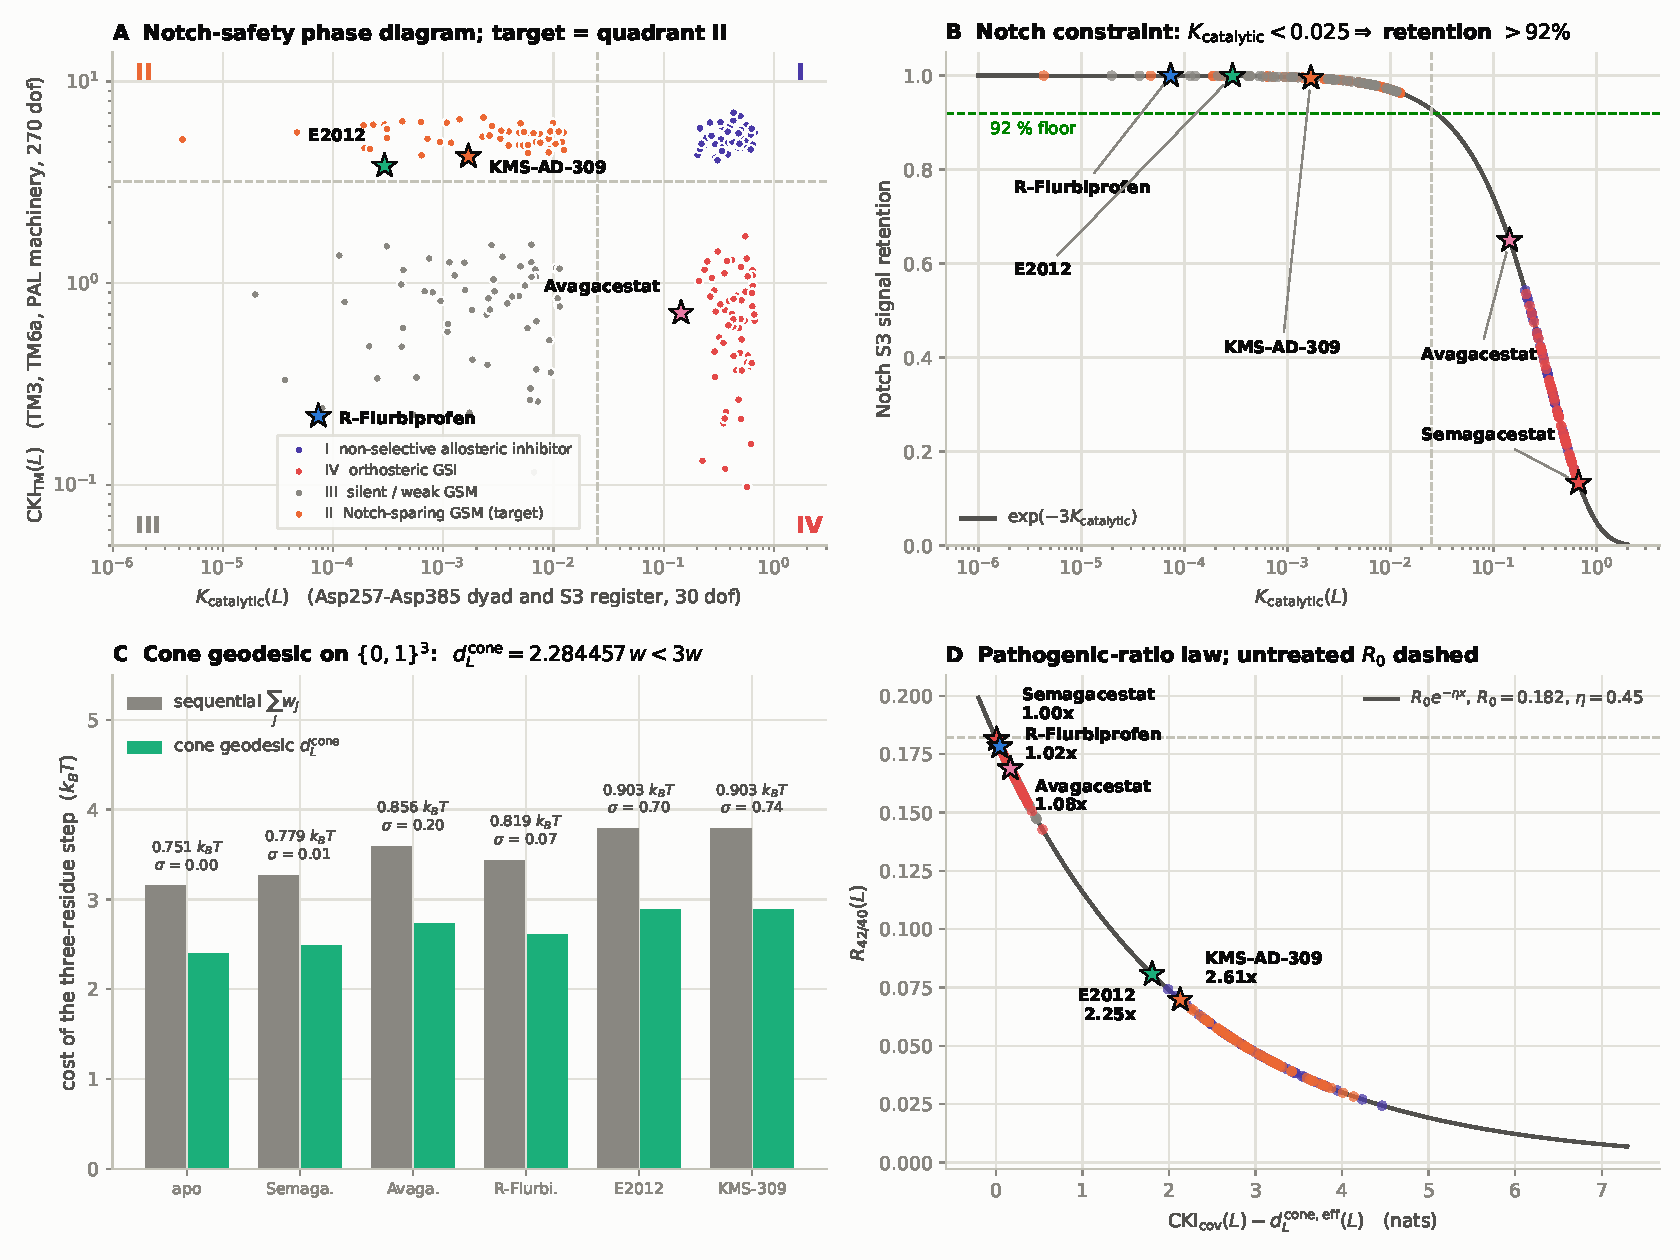
\includegraphics[width=\textwidth]{fig09_ad_gamma_secretase_gsm.pdf}
\caption{(A) The Notch-safety phase diagram: the $240$ screened ligands and the five reference compounds in the plane of Section~\ref{sec:intro}, with the thresholds $\Kcat=0.025$ and $\CKItm=3.20$ dashed. Quadrant~II is the target class. (B) The Notch constraint \eqref{eq:notch}: retention against $\Kcat$, with the $92\,\%$ floor. Semagacestat falls to $13.31\,\%$ and Avagacestat to $64.96\,\%$; the two modulators sit at the plateau. (C) The cone geodesic of Definition~\ref{def:cone} against the sequential cost, for the apo model and the five compounds, with the discount and the synchronous fraction $\sigma$. (D) The design-brief law \eqref{eq:ratio}; the dashed line is the untreated $R_0=0.182$.}
\label{fig:main}
\end{figure}

\begin{figure}[htbp]
\centering
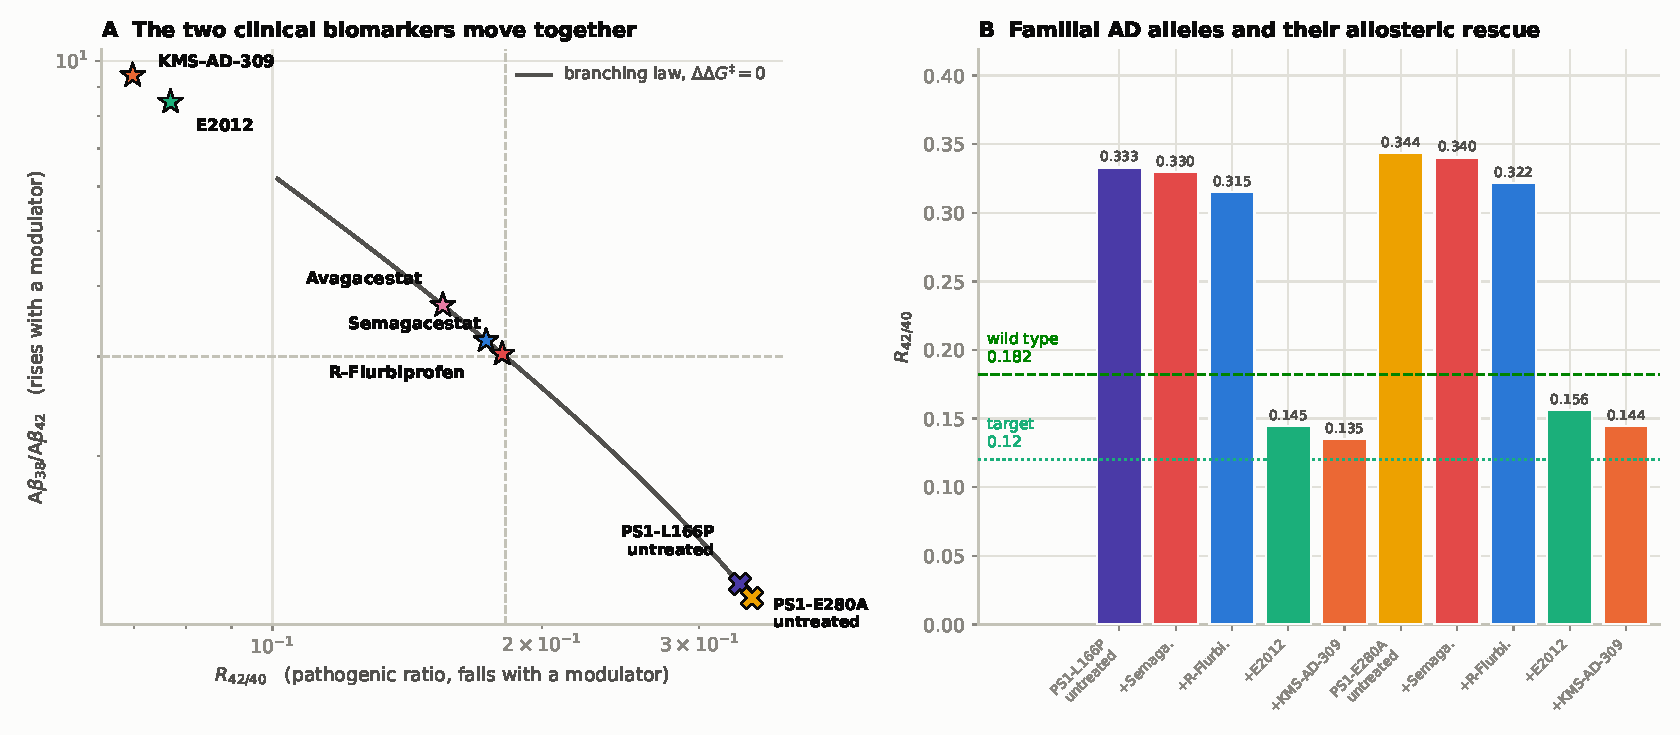
\includegraphics[width=\textwidth]{fig09b_biomarkers_and_fad_rescue.pdf}
\caption{(A) Proposition~\ref{prop:branch}: the two clinical biomarkers lie on one curve, on which a compound's position is fixed by $\Gamma$ alone, so they are one measurement seen twice rather than two. The two familial alleles (crosses) sit at the pathogenic end of the same curve, below the wild-type $\Ab_{38}/\Ab_{42}=\rho_0=3$ and to the right of $R_0=0.182$; the dashed lines mark those wild-type values. (B) Section~\ref{sec:fad}: each allele untreated and under each of the five compounds, against the wild-type baseline (dashed) and the stricter target $0.12$ (dotted). Only the two quadrant-II modulators cross the baseline.}
\label{fig:fad}
\end{figure}

\begin{table}[ht]
\centering\small
\caption{The three-zone model of Definition~\ref{def:model}. The stiffness is a weighted graph Laplacian plus a tether $t=0.9$; its spectrum is $[0.9000,\,24.8622]$ with condition number $27.62$ and $\dim\ker K=0$, as Proposition~\ref{prop:pd} requires. Inter-block couplings: gate--channel $1.0$, channel packing $1.2$, catalytic--channel $0.35$, catalytic--gate $0.25$.}
\label{tab:model}
\begin{tabular}{@{}l r p{58mm} r@{}}
\toprule
block & dof & segments (dof) & path stiffness \\
\midrule
catalytic $\mathcal{C}$ & $30$ & D257 loop ($8$), D385 loop ($8$), S3 register ($14$) & $6.0$ \\
gate $\mathcal{G}$ & $70$ & TM6a ($40$), PAL ($30$) & $4.0$ \\
channel $\mathcal{H}$ & $200$ & TM1--TM9 ($24$, $24$, $26$, $22$, $22$, $24$, $22$, $20$, $16$) & $5.0$ \\
\bottomrule
\end{tabular}
\end{table}

\begin{table}[ht]
\centering\footnotesize\setlength{\tabcolsep}{4pt}
\caption{Theorem~\ref{thm:schur}: the catalytic couplings are scaled by $s$ and the perturbation is held fixed at the purely allosteric ligand. $\|\Delta P\|_F$ is the change of the catalytic precision \eqref{eq:dP}; leakage is $\|\Delta\Sigma_{\CC\CC}\|_F/\|\Sigma_{\CC\CC}\|_F$. Asymptotic exponents fitted on $s\le0.125$: $1.9906$, $1.9709$, $1.9755$, $3.9633$, against the predicted $2,2,2,4$. Over the whole scan $\CKItm$ varies by a factor $1.0050$.}
\label{tab:schur}
\begin{tabular}{@{}r r r r r r r@{}}
\toprule
$s$ & $K_{\mathrm{cat,chan}}$ & $\|\Delta P\|_F$ & leakage & $D_{\mathrm{mean}}$ & $D_{\mathrm{cov}}$ & $\CKItm$ \\
\midrule
$0.03125$ & $0.01094$ & $1.58 \times 10^{-5}$ & $9.19 \times 10^{-7}$ & $2.11 \times 10^{-10}$ & $7.64 \times 10^{-13}$ & $4.2654$ \\
$0.06250$ & $0.02187$ & $6.32 \times 10^{-5}$ & $3.65 \times 10^{-6}$ & $8.38 \times 10^{-10}$ & $1.21 \times 10^{-11}$ & $4.2650$ \\
$0.12500$ & $0.04375$ & $2.51 \times 10^{-4}$ & $1.45 \times 10^{-5}$ & $3.30 \times 10^{-9}$ & $1.90 \times 10^{-10}$ & $4.2641$ \\
$0.25000$ & $0.08750$ & $9.94 \times 10^{-4}$ & $5.53 \times 10^{-5}$ & $1.28 \times 10^{-8}$ & $2.90 \times 10^{-9}$ & $4.2625$ \\
$0.50000$ & $0.17500$ & $3.89 \times 10^{-3}$ & $2.07 \times 10^{-4}$ & $4.85 \times 10^{-8}$ & $4.24 \times 10^{-8}$ & $4.2593$ \\
$1.00000$ & $0.35000$ & $1.49 \times 10^{-2}$ & $7.30 \times 10^{-4}$ & $1.74 \times 10^{-7}$ & $5.71 \times 10^{-7}$ & $4.2536$ \\
$2.00000$ & $0.70000$ & $5.48 \times 10^{-2}$ & $2.34 \times 10^{-3}$ & $5.72 \times 10^{-7}$ & $6.70 \times 10^{-6}$ & $4.2441$ \\
\bottomrule
\end{tabular}
\end{table}

\begin{table}[ht]
\centering\small\setlength{\tabcolsep}{5pt}
\caption{Theorem~\ref{thm:cone} and Numerical observation~\ref{obs:mono}: the anisotropy family \eqref{eq:family} at fixed $\sum_jw_j=3.15\,\kT$. The relative cost rises and the discount falls monotonically away from the isotropic point. Distances in $\kT$.}
\label{tab:cone}
\begin{tabular}{@{}r r r r r r r@{}}
\toprule
$a$ & $w_{\mathrm{TM3}}$ & $w_{\mathrm{TM6a}}$ & $w_{\mathrm{PAL}}$ & $\dcone$ & $\dcone/\sum_jw_j$ & discount \\
\midrule
$0.0$ & $1.0500$ & $1.0500$ & $1.0500$ & $2.39868$ & $0.761486$ & $0.75132$ \\
$0.1$ & $1.1550$ & $1.0500$ & $0.9450$ & $2.40137$ & $0.762341$ & $0.74863$ \\
$0.2$ & $1.2600$ & $1.0500$ & $0.8400$ & $2.40950$ & $0.764921$ & $0.74050$ \\
$0.3$ & $1.3650$ & $1.0500$ & $0.7350$ & $2.42320$ & $0.769270$ & $0.72680$ \\
$0.4$ & $1.4700$ & $1.0500$ & $0.6300$ & $2.44273$ & $0.775468$ & $0.70727$ \\
$0.5$ & $1.5750$ & $1.0500$ & $0.5250$ & $2.46846$ & $0.783639$ & $0.68154$ \\
$0.6$ & $1.6800$ & $1.0500$ & $0.4200$ & $2.50099$ & $0.793966$ & $0.64901$ \\
$0.7$ & $1.7850$ & $1.0500$ & $0.3150$ & $2.54119$ & $0.806727$ & $0.60881$ \\
$0.8$ & $1.8900$ & $1.0500$ & $0.2100$ & $2.59045$ & $0.822364$ & $0.55955$ \\
\bottomrule
\end{tabular}
\end{table}

\begin{table}[ht]
\centering\footnotesize\setlength{\tabcolsep}{3.5pt}
\caption{The five reference compounds: occupancy strengths, the two quadrant coordinates, the rotation part of the covariance term, the selectivity index \eqref{eq:snotch} and the quadrant. Retention is $100\,e^{-3\Kcat}$ per cent; the design floor is $92\,\%$ and the potency threshold is $3.20$. Note that $\Snotch$ ranks E2012 above the more potent lead, which is Proposition~\ref{prop:sat}.}
\label{tab:compa}
\begin{tabular}{@{}l r r r r r r r r c@{}}
\toprule
compound & $s_{\mathrm{cat}}$ & $s_{\mathrm{gate}}$ & $s_{\mathrm{chan}}$ & $\Kcat$ & ret.\ (\%) & $\CKItm$ & $D_{\mathrm{rot}}$ & $\Snotch$ & quad. \\
\midrule
Semagacestat & $1.000$ & $0.05$ & $0.05$ & $6.722 \times 10^{-1}$ & $13.31$ & $0.0344$ & $0.0286$ & $0.05104$ & IV \\
Avagacestat & $0.280$ & $0.32$ & $0.28$ & $1.438 \times 10^{-1}$ & $64.96$ & $0.7130$ & $0.6482$ & $4.924$ & IV \\
R-Flurbiprofen & $0.004$ & $0.18$ & $0.12$ & $7.342 \times 10^{-5}$ & $99.98$ & $0.2194$ & $0.1919$ & $204.4$ & III \\
E2012 & $0.008$ & $0.95$ & $0.92$ & $2.933 \times 10^{-4}$ & $99.91$ & $3.8176$ & $3.6400$ & $2952$ & II \\
KMS-AD-309 & $0.020$ & $1.00$ & $1.00$ & $1.688 \times 10^{-3}$ & $99.49$ & $4.2536$ & $4.0433$ & $1583$ & II \\
\bottomrule
\end{tabular}
\end{table}

\begin{table}[ht]
\centering\footnotesize\setlength{\tabcolsep}{3.5pt}
\caption{The same compounds in the cone geometry. Step weights from \eqref{eq:weights}, the cone distance of Definition~\ref{def:cone}, the synchronous fraction \eqref{eq:sigma}, the barrier discount \eqref{eq:clamp} in kcal/mol with the corresponding rate factor for the $\Ab_{42}\to\Ab_{38}$ step, and the design-brief law \eqref{eq:ratio} with its fold reduction against $R_0=0.182$. Weights and distances in $\kT$.}
\label{tab:compb}
\begin{tabular}{@{}l r r r r r r r r r r@{}}
\toprule
compound & $w_{\mathrm{TM3}}$ & $w_{\mathrm{TM6a}}$ & $w_{\mathrm{PAL}}$ & $\sum_jw_j$ & $\dcone$ & $\sigma$ & $\Delta\Delta G^{\ddagger}$ & $k$-fold & $R_{42/40}$ & fold \\
\midrule
Semagacestat & $1.1026$ & $1.0794$ & $1.0860$ & $3.2680$ & $2.4886$ & $0.0107$ & $0.0051$ & $1.008$ & $0.18136$ & $1.004$ \\
Avagacestat & $1.2331$ & $1.1603$ & $1.1954$ & $3.5888$ & $2.7331$ & $0.1997$ & $0.1053$ & $1.186$ & $0.16883$ & $1.078$ \\
R-Flurbiprofen & $1.1568$ & $1.1255$ & $1.1506$ & $3.4330$ & $2.6142$ & $0.0663$ & $0.0334$ & $1.056$ & $0.17826$ & $1.021$ \\
E2012 & $1.3049$ & $1.2090$ & $1.2731$ & $3.7871$ & $2.8843$ & $0.6967$ & $0.3876$ & $1.876$ & $0.08075$ & $2.254$ \\
KMS-AD-309 & $1.3022$ & $1.2097$ & $1.2750$ & $3.7869$ & $2.8841$ & $0.7353$ & $0.4090$ & $1.942$ & $0.06978$ & $2.608$ \\
\bottomrule
\end{tabular}
\end{table}

\begin{table}[ht]
\centering\footnotesize\setlength{\tabcolsep}{4.5pt}
\caption{Proposition~\ref{prop:branch}: the two clinical biomarkers from one branching partition, with $\rho_0=3.00$ and $\eta_{\mathrm{clamp}}=0.22620$. ``$\times$WT'' is $\Ab_{38}/\Ab_{42}$ relative to the wild-type $\rho_0$, ``fold'' is $R_0/R_{42/40}$. The last column is the disagreement with the one-constant design-brief law of Table~\ref{tab:compb}; the calibration anchor is KMS-AD-309.}
\label{tab:biomark}
\begin{tabular}{@{}l r r r r r r r@{}}
\toprule
compound & $\Gamma$ & $\Delta\Delta G^{\ddagger}$ & $\Ab_{38}/\Ab_{42}$ & $\times$WT & $R_{42/40}$ & fold & gap (\%) \\
\midrule
Semagacestat & $+0.0078$ & $+0.0051$ & $3.0304$ & $1.010$ & $0.18063$ & $1.008$ & $0.41$ \\
Avagacestat & $+0.1669$ & $+0.1053$ & $3.6961$ & $1.232$ & $0.15502$ & $1.174$ & $8.91$ \\
R-Flurbiprofen & $+0.0461$ & $+0.0334$ & $3.2005$ & $1.067$ & $0.17331$ & $1.050$ & $2.86$ \\
E2012 & $+1.8059$ & $+0.3876$ & $8.4661$ & $2.822$ & $0.07691$ & $2.367$ & $5.00$ \\
KMS-AD-309 & $+2.1303$ & $+0.4090$ & $9.4339$ & $3.145$ & $0.06977$ & $2.608$ & $0.01$ \\
\bottomrule
\end{tabular}
\end{table}

\begin{table}[ht]
\centering\footnotesize\setlength{\tabcolsep}{4pt}
\caption{The screen of $240$ ligands, sixty sampled for each quadrant. ``Assay'' counts hits of the catalytic activity read-out, $\Kcat>0.025$; ``both'' counts ligands meeting both design constraints. Retention in per cent.}
\label{tab:screen}
\begin{tabular}{@{}c r r r r r r r r r@{}}
\toprule
quadrant & $n$ & $\Kcat$ min & $\Kcat$ max & $\CKItm$ min & $\CKItm$ max & ret.\ min & ret.\ max & assay & both \\
\midrule
I & $60$ & $2.04 \times 10^{-1}$ & $6.70 \times 10^{-1}$ & $4.071$ & $7.001$ & $13.39$ & $54.30$ & $60$ & $0$ \\
II & $60$ & $4.29 \times 10^{-6}$ & $1.24 \times 10^{-2}$ & $4.308$ & $6.640$ & $96.34$ & $100.00$ & $0$ & $60$ \\
III & $60$ & $1.96 \times 10^{-5}$ & $1.14 \times 10^{-2}$ & $0.115$ & $1.553$ & $96.63$ & $99.99$ & $0$ & $0$ \\
IV & $60$ & $2.09 \times 10^{-1}$ & $6.71 \times 10^{-1}$ & $0.098$ & $1.710$ & $13.35$ & $53.50$ & $60$ & $0$ \\
\bottomrule
\end{tabular}
\end{table}

\begin{table}[ht]
\centering\footnotesize\setlength{\tabcolsep}{4.5pt}
\caption{Section~\ref{sec:fad}: two familial PSEN1 alleles, modelled as a loss of gate and channel stiffness, and the effect of each compound on them. ``fold'' is the reduction of $R_{42/40}$ against the untreated allele; retention is measured against the untreated allele, so it is the Notch inhibition the drug \emph{adds}. The last column is the occupancy multiplier at which $R_{42/40}$ reaches $0.12$. The wild-type baseline is $R_0=0.182$.}
\label{tab:fad}
\begin{tabular}{@{}l l r r r r r r@{}}
\toprule
allele & compound & $\Gamma$ & $\Ab_{38}/\Ab_{42}$ & $R_{42/40}$ & fold & ret.\ (\%) & $m^\ast$ \\
\midrule
PS1-L166P & untreated & $-1.9682$ & $1.1861$ & $0.33301$ & $1.00$ & $100.00$ & -- \\
 & Semagacestat & $-1.9537$ & $1.2083$ & $0.32967$ & $1.01$ & $13.30$ & $>4$ \\
 & Avagacestat & $-1.6395$ & $1.6479$ & $0.27493$ & $1.21$ & $64.94$ & $3.689$ \\
 & R-Flurbiprofen & $-1.8901$ & $1.3118$ & $0.31491$ & $1.06$ & $99.98$ & $>4$ \\
 & E2012 & $+0.4379$ & $4.0332$ & $0.14464$ & $2.30$ & $99.91$ & $1.188$ \\
 & KMS-AD-309 & $+0.7068$ & $4.3853$ & $0.13518$ & $2.46$ & $99.49$ & $1.112$ \\
\midrule
PS1-E280A & untreated & $-2.1419$ & $1.1189$ & $0.34357$ & $1.00$ & $100.00$ & -- \\
 & Semagacestat & $-2.1275$ & $1.1400$ & $0.34019$ & $1.01$ & $13.31$ & $>4$ \\
 & Avagacestat & $-1.8393$ & $1.5301$ & $0.28773$ & $1.19$ & $64.96$ & $3.981$ \\
 & R-Flurbiprofen & $-2.0452$ & $1.2634$ & $0.32164$ & $1.07$ & $99.98$ & $>4$ \\
 & E2012 & $+0.1476$ & $3.6586$ & $0.15627$ & $2.20$ & $99.91$ & $1.244$ \\
 & KMS-AD-309 & $+0.4695$ & $4.0428$ & $0.14436$ & $2.38$ & $99.49$ & $1.153$ \\
\bottomrule
\end{tabular}
\end{table}



\clearpage

%%%%%%%%%%%%%%%%%%%%%%%%%%%%%%%%%%%%%%%%%%%%%%%%%%%%%%%%%%%%%%%%%%%%%%%%%%%%%%%
\section{Assessment, limits and open problems}
\label{sec:assess}

\subsection{What was established}
Table~\ref{tab:assess} summarises the status of each claim: whether it is proved, and where it is checked.

\begin{table}[ht]
\centering\small\setlength{\tabcolsep}{5pt}
\caption{Status of the claims. ``Proved'' means proved here for the model of Definition~\ref{def:model}; ``numerical'' means verified computationally and not proved.}
\label{tab:assess}
\begin{tabular}{@{}l l l@{}}
\toprule
claim & status & evidence \\
\midrule
$\lambda_{\min}(K)=t$ exactly & proved & Prop.~\ref{prop:pd}; $0.9000$ measured \\
catalytic precision is bilinear in $K_{\CC\MM}$ & proved & Thm~\ref{thm:schur}(i), Eq.~\eqref{eq:dP} \\
leakage and mean term are $O(s^2)$ & proved & Thm~\ref{thm:schur}(ii)--(iii); $1.97$, $1.98$ \\
covariance term is $O(s^4)$ & proved & Thm~\ref{thm:schur}(iii); $3.96$ \\
$\CKItm$ is screening-independent & proved & Thm~\ref{thm:schur}(iv); factor $1.0050$ \\
equal-weight closed form & proved & Thm~\ref{thm:cone}(ii); error $4.44\times10^{-16}$ \\
$\max_jw_j\le\dcone<\sum_jw_j$ & proved & Thm~\ref{thm:cone}(iii); $243/243$ \\
anisotropy family is even in $a$ & proved & Prop.~\ref{prop:even}; error $0$ \\
isotropy minimises $\dcone$ at fixed sum & numerical & Obs.~\ref{obs:mono}; $2001$ points \\
well-posedness of the recursion & numerical & Eq.~\eqref{eq:slack}; margin $\ge7.2\times10^{-5}$ \\
$\Snotch$ saturates at $\CKItm/\varepsilon_0$ & proved & Prop.~\ref{prop:sat}; max ratio $0.9957$ \\
two biomarkers from one partition & proved & Prop.~\ref{prop:branch}; exact for the model \\
design-brief law is the $\rho\gg1$ limit & proved & Eq.~\eqref{eq:limit}; gap $\le8.91\,\%$ \\
assay recall on quadrant~II is zero & definitional & Prop.~\ref{prop:anti}(i) \\
quadrant~II is non-empty and reachable & numerical & Prop.~\ref{prop:anti}(ii); $60/240$ \\
FAD alleles loosen rather than activate & modelled & \S\ref{sec:fad}; $\zeta=-1$, $R$ to $0.33$--$0.34$ \\
quadrant~II modulators reverse the sign & numerical & Table~\ref{tab:fad}; $\Gamma>0$ on both alleles \\
inhibitors do not rescue familial disease & numerical & Table~\ref{tab:fad}; $1.01\times$ at $13\,\%$ Notch \\
\bottomrule
\end{tabular}
\end{table}

\subsection{Limits}
We state five, in the order in which they would bite.

\textbf{(a) The dynamics are a harmonic surrogate, and the structures fix topology only.} The model is a Gaussian elastic network on a \emph{schematic} contact graph. What Section~\ref{sec:cryoem} takes from \texttt{6IYC}, \texttt{6IDF} and \texttt{7D8X} is which parts exist and how they are wired: the aspartates on TM6 and TM7, the hybrid $\beta$-sheet register, the TM6a/PAL gate, the nine-helix horseshoe. No coordinates are used, nothing is docked, no free energy is computed, and the model is not molecular dynamics. In particular it does \emph{not} place E2012 at the extracellular allosteric site that \texttt{7D8X} resolves; it represents a modulator by the gate--channel coupling it induces, which is a consequence rather than a pose. Every quantity reported is a property of Definition~\ref{def:model}.

\textbf{(b) The compounds enter through their class, not their chemistry.} All five are represented by the triple $(s_{\mathrm{cat}},s_{\mathrm{gate}},s_{\mathrm{chan}})$ and by nothing else, and those triples were chosen to encode the pharmacological class each compound is known to belong to. The model then reproduces the clinical separation of two inhibitors, a weak modulator, a second-generation modulator and a designed lead; it does not predict that separation from structure, and it could not, because the map from a molecule to its triple is exactly what is missing. The same caveat applies to the two alleles of Section~\ref{sec:fad}, whose softening factors encode ``severe loss of gate stiffness'' rather than any calculation from the mutation.

\textbf{(c) \lead{} is a designed point, not a compound.} It is a location in the parameter space of Definition~\ref{def:model} chosen to satisfy the design brief. No synthesis, no assay, no measurement.

\textbf{(d) Three constants are calibrated, and one target was used to set the allele severity.} In \eqref{eq:ratio}, $R_0=0.182$ and $\eta=0.45$ are phenomenological. In the branching law, $\rho_0=3.00$ is a biochemical input and $\eta_{\mathrm{clamp}}=0.22620$ is fitted on one anchor. The severity of the two alleles was chosen so that their untreated $R_{42/40}$ lands in the reported $0.33$--$0.36$ range; that range is therefore an input, not a result. What was \emph{not} fitted is the sign of the alleles' effect, the co-movement of the two biomarkers, the rescue, or any quadrant assignment, none of which depends on these constants.

\textbf{(e) The interesting number is the zero, not the hundred per cent.} The screen's $100\,\%$ quadrant agreement says only that the sampled strength ranges realise their intended quadrants; it is a design check on the sampler, not a validation of any classifier against experiment. The informative statement is Proposition~\ref{prop:anti}, and within it the conjunction of (ii) and (iii) rather than (i).

\subsection{Open problems}
\begin{enumerate}[label=\textup{(\arabic*)},leftmargin=2.4em,itemsep=4pt]
\item\label{op:schur} \emph{Schur-convexity of the cone distance.} Prove or disprove that $\dcone$ is a convex function of $w$ on $(0,\infty)^k$. By symmetry this would upgrade Numerical observation~\ref{obs:mono} to a theorem valid for every direction, not merely along the family \eqref{eq:family}, and would establish isotropic optimality of the cooperativity discount in general.
\item \emph{The degenerate regime of the recursion.} Definition~\ref{def:cone} presupposes \eqref{eq:slack}. Characterise the set of weights where it fails, and extend the recursion by replacing the summand with its positive part. The family \eqref{eq:family} approaches the boundary as $a\to1$, where the margin falls to $7.2\times10^{-5}$.
\item \emph{Calibrating the branching law.} Determine $\rho_0$ and $\eta_{\mathrm{clamp}}$ from cell-based $\Ab$ profiling of a compound series with independently measured channel rearrangement, rather than fitting one of them on a single anchor. Proposition~\ref{prop:branch} makes a falsifiable prediction for such a series: every compound must lie on one curve in the $(R_{42/40},\,\Ab_{38}/\Ab_{42})$ plane, with no free parameter per compound.
\item \emph{Real ensembles.} Rebuild Definition~\ref{def:model} on \texttt{6IYC} or \texttt{7D8X} with molecular-dynamics ensembles, using the estimators of Papers~VII--VIII, and test whether the Schur exponent of Theorem~\ref{thm:schur} survives contact with a real coupling block. The same rebuild would let the FAD alleles be introduced as actual substitutions rather than as softening factors, which is the weakest point of Section~\ref{sec:fad}.
\item \emph{The missing map.} Learn the map from a molecule to $(s_{\mathrm{cat}},s_{\mathrm{gate}},s_{\mathrm{chan}})$. Without it the framework classifies ligands it is given but cannot propose them, and Limit~(b) remains the binding constraint on the whole programme.
\end{enumerate}

\subsection*{Data and code availability}
Everything in this paper is produced by two scripts in \texttt{code/}:
\begin{itemize}[leftmargin=1.6em,itemsep=2pt]
\item \texttt{exp09\_ad\_gamma\_secretase\_gsm.py}, the experiment;
\item \texttt{exp09\_lib.py}, its model library;
\item \texttt{paper09\_compute\_tables.py}, the companion that writes the table bodies.
\end{itemize}
The four data files are in \texttt{data/}, the two figures in \texttt{figures/} and the logs in \texttt{results/}. The package \pkg{} is inherited unchanged from Papers~VII--VIII. Twenty model unit tests and the twelve inherited package tests pass.

\subsection*{Funding}
This project was supported by the National Natural Science Foundation of China (No.~22464010), the Guangxi Natural Science Foundation of China (No.~2025GXNSFAA069294), and the 2025 Bagui Youth Top Talent Project.

%%%%%%%%%%%%%%%%%%%%%%%%%%%%%%%%%%%%%%%%%%%%%%%%%%%%%%%%%%%%%%%%%%%%%%%%%%%%%%%
\begin{thebibliography}{99}
\bibitem{Aronsson2004} G.~Aronsson, M.~G. Crandall and P.~Juutinen, \emph{A tour of the theory of absolutely minimizing functions}, Bull. Amer. Math. Soc. \textbf{41} (2004), 439--505.
\bibitem{Atilgan2001} A.~R. Atilgan, S.~R. Durell, R.~L. Jernigan, M.~C. Demirel, O.~Keskin and I.~Bahar, \emph{Anisotropy of fluctuation dynamics of proteins with an elastic network model}, Biophys. J. \textbf{80} (2001), 505--515.
\bibitem{Bhattacharyya1943} A.~Bhattacharyya, \emph{On a measure of divergence between two statistical populations defined by their probability distributions}, Bull. Calcutta Math. Soc. \textbf{35} (1943), 99--109.
\bibitem{Chen2026} R.~Chen, \emph{Localized Bost--Connes systems}, monograph, 2026, DOI 10.5281/zenodo.22883179.
\bibitem{ChenChen2026I} Z.~Chen and R.~Chen, \emph{Statistical pharmacology via Kakutani dichotomy I: the marginal drug Kakutani index and the $\alpha_c=1/2$ criticality theorem in high-dimensional conformational ensembles}, 2026, DOI 10.5281/zenodo.23005921.
\bibitem{ChenChen2026II} Z.~Chen and R.~Chen, \emph{Statistical pharmacology via Kakutani dichotomy II: the correlated Kakutani index, the 99.95\% covariance dominance theorem, and spectral fingerprints of cryptic allostery}, 2026, DOI 10.5281/zenodo.23012217.
\bibitem{ChenChen2026III} Z.~Chen and R.~Chen, \emph{Statistical pharmacology via Kakutani dichotomy III: spectral Kakutani--Feldman--H\'ajek criticality of correlated conformational modes}, 2026, DOI 10.5281/zenodo.23015709.
\bibitem{ChenChen2026IV} Z.~Chen and R.~Chen, \emph{Statistical pharmacology via Kakutani dichotomy IV: KMS inverse-temperature criticality $\beta_c=1$, pocket-to-distal tail allostery, and the four-quadrant ligand classification}, 2026, DOI 10.5281/zenodo.23018236.
\bibitem{ChenChen2026V} Z.~Chen and R.~Chen, \emph{Statistical pharmacology via Kakutani dichotomy V: the chemical obstruction group, Borel--Cantelli tail order parameters, and the relative-entropy staircase}, 2026, DOI 10.5281/zenodo.23027704.
\bibitem{ChenChen2026VI} Z.~Chen and R.~Chen, \emph{Statistical pharmacology via Kakutani dichotomy VI: Wasserstein phase separation, the single-step scan barrier, and cone-geodesic collective moves}, 2026, DOI 10.5281/zenodo.23029360.
\bibitem{ChenChen2026VII} Z.~Chen and R.~Chen, \emph{Statistical pharmacology via Kakutani dichotomy VII: the kakutani\_pharma pipeline, Ledoit--Wolf regularized CKI, split-trajectory null subtraction, and shell-scaling exponents in multi-domain allostery}, 2026, DOI 10.5281/zenodo.23039869.
\bibitem{ChenChen2026VIII} Z.~Chen and R.~Chen, \emph{Statistical pharmacology via Kakutani dichotomy VIII: empirical validation on experimental all-atom protein ensembles, influence-function block selection, and bootstrap coverage calibration}, 2026, DOI 10.5281/zenodo.23045772.
\bibitem{ChenChen2026S} Z.~Chen and R.~Chen, \emph{Kakutani--KMS theory of ligand-induced conformational phase transitions}, 2026, DOI 10.5281/zenodo.23042828.
\bibitem{Coric2012} V.~Coric, C.~H. van~Dyck, S.~Salloway, N.~Andreasen, M.~Brody, R.~W. Richter, H.~Soininen, S.~Thein, T.~Shiovitz, G.~Pilcher, S.~Colby, L.~Rollin, R.~Dockens, C.~Pachai, E.~Portelius, U.~Andreasson, K.~Blennow, H.~Soares, C.~Albright, H.~H. Feldman and R.~M. Berman, \emph{Safety and tolerability of the $\gamma$-secretase inhibitor avagacestat in a phase 2 study of mild to moderate Alzheimer disease}, Arch. Neurol. \textbf{69} (2012), 1430--1440.
\bibitem{DeStrooper2010} B.~De~Strooper, \emph{Proteases and proteolysis in Alzheimer disease: a multifactorial view on the disease process}, Physiol. Rev. \textbf{90} (2010), 465--494.
\bibitem{Doody2013} R.~S. Doody et~al., \emph{A phase 3 trial of semagacestat for treatment of Alzheimer's disease}, N. Engl. J. Med. \textbf{369} (2013), 341--350.
\bibitem{Green2009} R.~C. Green et~al., \emph{Effect of tarenflurbil on cognitive decline and activities of daily living in patients with mild Alzheimer disease}, JAMA \textbf{302} (2009), 2557--2564.
\bibitem{Horn1985} R.~A. Horn and C.~R. Johnson, \emph{Matrix Analysis}, Cambridge University Press, 1985.
\bibitem{Kakutani1948} S.~Kakutani, \emph{On equivalence of infinite product measures}, Ann. of Math. \textbf{49} (1948), 214--224.
\bibitem{Marshall2011} A.~W. Marshall, I.~Olkin and B.~C. Arnold, \emph{Inequalities: Theory of Majorization and Its Applications}, 2nd ed., Springer, New York, 2011.
\bibitem{Takami2009} M.~Takami, Y.~Nagashima, Y.~Sano, S.~Ishihara, M.~Morishima-Kawashima, S.~Funamoto and Y.~Ihara, \emph{$\gamma$-Secretase: successive tripeptide and tetrapeptide release from the transmembrane domain of $\beta$-carboxyl terminal fragment}, J. Neurosci. \textbf{29} (2009), 13042--13052.
\bibitem{Weggen2001} S.~Weggen, J.~L. Eriksen, P.~Das, S.~A. Sagi, R.~Wang, C.~U. Pietrzik, K.~A. Findlay, T.~E. Smith, M.~P. Murphy, T.~Bulter, D.~E. Kang, N.~Marquez-Sterling, T.~E. Golde and E.~H. Koo, \emph{A subset of NSAIDs lower amyloidogenic $\mathrm{A}\beta_{42}$ independently of cyclooxygenase activity}, Nature \textbf{414} (2001), 212--216.
\bibitem{Wolfe1999} M.~S. Wolfe, W.~Xia, B.~L. Ostaszewski, T.~S. Diehl, W.~T. Kimberly and D.~J. Selkoe, \emph{Two transmembrane aspartates in presenilin-1 required for presenilin endoproteolysis and $\gamma$-secretase activity}, Nature \textbf{398} (1999), 513--517.
\bibitem{Yang2019} G.~Yang, R.~Zhou, Q.~Zhou, X.~Guo, C.~Yan, M.~Ke, J.~Lei and Y.~Shi, \emph{Structural basis of Notch recognition by human $\gamma$-secretase}, Nature \textbf{565} (2019), 192--197. PDB \texttt{6IDF}.
\bibitem{Yang2021} G.~Yang, R.~Zhou, X.~Guo, C.~Yan, J.~Lei and Y.~Shi, \emph{Structural basis of $\gamma$-secretase inhibition and modulation by small molecule drugs}, Cell \textbf{184} (2021), 521--533.e14. PDB \texttt{7D8X} ($\gamma$-secretase with E2012 and L685,458).
\bibitem{Zhou2019} R.~Zhou, G.~Yang, X.~Guo, Q.~Zhou, J.~Lei and Y.~Shi, \emph{Recognition of the amyloid precursor protein by human $\gamma$-secretase}, Science \textbf{363} (2019), eaaw0930. PDB \texttt{6IYC}.
\end{thebibliography}

\end{document}
